\documentclass{article}

\usepackage{times}
\usepackage{uist}
\usepackage[colorlinks=true,linkcolor=black, citecolor=black,bookmarks=true,pdfauthor={Jon Noronha, Eric Hysen, Haoqi Zhang, and Krzysztof Z. Gajos},pdftitle={PlateMate: Crowdsourcing Nutrition Analysis from Food Photographs}]{hyperref}
\usepackage{graphics}
\usepackage{graphicx}
\usepackage[usenames,dvipsnames]{color}
\usepackage{subfigure}
\usepackage{url}


\begin{document}

% --- Copyright notice ---
\conferenceinfo{UIST'11}{October 16-19, 2011, Santa Barbara, CA, USA}
\CopyrightYear{2011}
\crdata{978-1-4503-0716-1/11/10}

% Uncomment the following line to hide the copyright notice
% \toappear{}
% ------------------------

%\bibliographystyle{plain}

\title{PlateMate: Crowdsourcing Nutrition Analysis from Food Photographs}

%%
%% Note on formatting authors at different institutions, as shown below:
%% Change width arg (currently 7cm) to parbox commands as needed to
%% accommodate widest lines, taking care not to overflow the 17.8cm line width.
%% Add or delete parboxes for additional authors at different institutions. 
%% If additional authors won't fit in one row, you can add a "\\"  at the
%% end of a parbox's closing "}" to have the next parbox start a new row.
%% Be sure NOT to put any blank lines between parbox commands!
%%

\author{
\parbox[t]{12cm}{\centering
	     {\em Jon Noronha, Eric Hysen, Haoqi Zhang, Krzysztof Z. Gajos}\\
	     Harvard School of Engineering and Applied Sciences\\
	   	33 Oxford St.,
	     Cambridge, MA 02138, USA\\
	     \{noronha,hysen,hqz,kgajos\}@seas.harvard.edu}
}

%% \author{
%% \parbox[t]{9cm}{\centering
%% 	     {\em Submission 433}\\
%% 	    }
%% }

\maketitle

\newcommand{\bug}
    {\mbox{\rule{2mm}{2mm}}}
\newcommand{\Bug}[1]
    {\bug \footnote{BUG: {#1}}}
    
\newcommand{\fix}[1]{\marginpar{\centering \textcolor{Magenta}{** FIX **}}{\color{Magenta}#1}}
\newcommand{\newcontent}[1]{#1}
\newcommand{\cut}[1]{\marginpar{\centering \textcolor{Red}{CUT? **}}{\color{Red}#1}}


\abstract We introduce PlateMate, a system that allows users to take photos of their meals and
receive estimates of food intake and composition. Accurate awareness
of this information can help people monitor their progress towards  
 dieting goals, but current
methods for food logging via self-reporting, expert observation, or
algorithmic analysis are time-consuming, expensive, or inaccurate.
PlateMate crowdsources nutritional analysis from photographs using
Amazon Mechanical Turk, automatically coordinating untrained workers
to estimate a meal's calories, fat, carbohydrates, and protein.  We
present the Management framework for crowdsourcing complex tasks,
which supports PlateMate's nutrition analysis workflow. Results of our evaluations
show that PlateMate is nearly as accurate as a trained
dietitian and easier to use for most users than traditional
self-reporting.
%\fix{propose drop: ``while remaining robust for general use across a wide
%variety of meal types.'' -- especially given problem with certain types such as soups.}

\classification{H5.2 [Information interfaces and presentation]:
User Interfaces. - Graphical user interfaces.}

\terms{Design, Human Factors}

\keywords{Human computation, Crowdsourcing, Mechanical Turk, Nutrition, Remote Food Photography}

  % makes some lines with lots of white space, but 	
  % tends to prevent words from sticking out in the margin
\tolerance=4000 
% these lines help eliminate widows/orphans
\widowpenalty=10000
\clubpenalty=10000

\interfootnotelinepenalty=10000

\section{INTRODUCTION}

%Everyone wants a nutritious diet,
%\fix{[in the citation here it says that only 2 out of 10 people want to improve their diet -- so it's hard to say everyone wants a nutritious diet when this is the case..]} 
%but 
The majority of Americans perceive
healthy eating as complicated~\cite{dinkins2000beliefs}.  Seeking
comprehensible and actionable advice, Americans spend over \$40
billion each year on diets and self-help
books~\cite{reisner08:diet},
%\cite{hoffmann05:costly,reisner08:diet}, 
%\fix{[Is the first citation a Forbes.com article? I couldn't access it.]} 
but achieve little
success: the majority eventually regain any lost weight and
more~\cite{mann2007medicare}.

%Everyone wants a nutritious diet, but healthy eating is hard. New
%Years resolutions flounder while more and more miracle diets
%proliferate each year. Restaurants and grocery stores capitalize on
%these challenges with low-fat menus and healthy-choice aisles, but
%little seems to change.  Part of the problem is that people lack
%information. They have no systematic record of what they are eating
%or what it was made of. This information is not sufficient for
%healthier eating, but it seems to be a necessary
%prerequisite~\cite{worsley2002nutrition}.

There are many factors that may impact successful long-term change in
eating habits.  \newcontent{Our work is based on the observation that
  food intake monitoring is a popular component of many diets.  For
  people who make a commitment to changing their eating habits,
  accurate logs of what they eat may help in monitoring progress
  toward set goals~\cite{locke02:building}.  Currently, food logging
  is typically done by hand using paper diaries, spreadsheets, or a
  growing number of specialized applications.}  This process is both
time-consuming and
error-prone~\cite{pikholz2004under,goris2000undereating}.
Nutritionists have explored alternative methods such as daily
interviews with trained experts. While these methods improve accuracy,
they are costly and still require substantial time investment.


%There are many factors that impact successful long-term behavior
%change.  Our work is based on the observation that maintaining
%accurate awareness of nutritional intake is a prerequisite for
%changing eating
%habits~\cite{worsley2002nutrition,baker1993self}. Indeed, most diets
%require followers to track their meals, and people typically do so
%with pen and paper or computer spreadsheets.  This process is both
%time-consuming and
%error-prone~\cite{pikholz2004under,goris2000undereating}.
%Nutritionists have explored alternative methods such as daily
%interviews with trained experts. These methods improve accuracy, but
%they are costly and still require substantial time investment.

Our work is inspired by the \emph{Remote Food Photography Method} (RFPM)~\cite{martin2009novel}, a novel approach from the nutrition literature. Rather
than remembering foods or writing down records, users take
\newcontent{two photographs of each meal: one at the beginning
  of the meal and one at the end documenting the leftovers.}
These images are analyzed by a third party, making logging easier and
discouraging self-deception. The challenge is in finding a qualified
third party without prohibitive costs. Expert nutritionists are 
scarce and costly, limiting the system to wealthy users or patients with
particular conditions.

To make accurate food logging easier and more affordable, we introduce
\emph{PlateMate}, a system for crowdsourcing nutritional analysis
(calories, fat, carbohydrates, and protein) from photographs of meals
using Amazon Mechanical Turk.
%PlateMate automatically coordinates untrained workers to estimate a meal's calories, fat, carbohydrates, and protein from a photograph. 
Complex tasks like this are hard problems for
crowdsourcing, as workers may vary drastically in experience and
reliability. To achieve accurate estimates, we propose a workflow in 
which the overall problem is decomposed into
small, manageable, and verifiable steps.
%\fix{perhaps note right here that we focus on estimating nutritional information under the assumption that the user eats what he or she photographs, and leave handling leftovers for future work? If do so here then drop next sentence maybe.} 
PlateMate uses this workflow to assign tasks to contributors, to validate and combine results, and to appropriately route tasks for further processing.
%\fix{tried to edit the text here some to be more specific as to what is assigned, validated, combined, routed --- some more specificity may help even more}
%Tasks are assigned,
%validated, combined, and appropriately routed through a larger
%workflow.

This paper makes three main contributions:
%\vspace*{-2mm}
\begin{enumerate}
\item We present PlateMate, an end-to-end system for crowdsourced nutrition analysis from food photographs.
\item We discuss the results of a two-part evaluation, which suggests
  PlateMate can be as accurate as experts and self-report methods, and
  more usable than manual logging for everyday use.
\newcontent{\item We introduce the Management framework---inspired by the structure of human organizations, it provides effective support for managing crowdsourcing of complex heterogeneous tasks.  }
% by coordinating contributions using a hierarchical message-passing system.}
\end{enumerate}
%\vspace*{-2mm}

%PlateMate implements the first of the two steps of the Remote Food
%Photography Method, that is, it performs nutrition analysis based on
%measurements of photographs of original portions. While the system can
%also be used on photographs of leftovers, other approaches that employ
%information obtained from measuring original portions in the process
%of measuring leftovers are possible and may actually be more efficient
%for the second step. In some situations, the second step may involve
%additional challenges, e.g., as caused by messy leftover plates where
%foods lose their original textual and shape and may thus be hard to
%identify.  Given that the first step is necessary for the RFPM method
%and that results from evaluating PlateMate will provide useful lessons
%for designing for the second step, for simplicity we focus on
%measuring original portions and leave handling of food waste for
%future work.

PlateMate implements the first step in the Remote Food Photography Method.  In the last section we suggest how it can be extended to also support the second step: the analysis of photographs of food waste.
 
In the next section we review relevant prior work.  We then describe
the design and implementation of the PlateMate system and its
components. Next, we discuss our Management framework.
We then present an evaluation of the accuracy and usability of
PlateMate and discuss the results. Finally, we consider future
extensions to PlateMate.

\begin{figure*}[t]
\begin{center}
   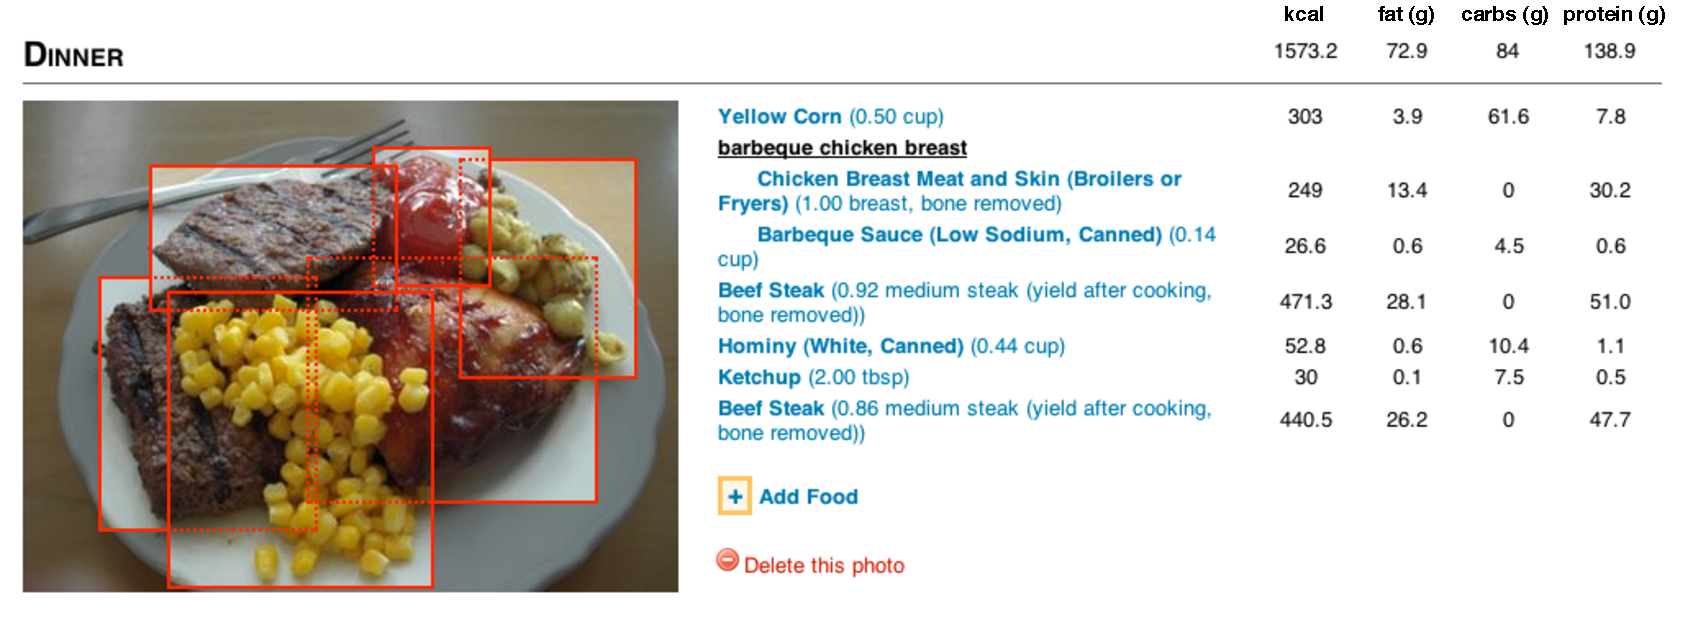
\includegraphics[width=\linewidth]{figs/ui-withHeaders.pdf}
   \caption{The PlateMate user interface.  Users upload photographs of their meals, which are processed through Mechanical Turk to produce a list of foods, serving sizes, and nutrition information.}
   \label{fig:ui}
\end{center}
\end{figure*}

\section{RELATED WORK}

%Prior work makes clear that eating depends on a variety of
%environmental and personal factors, with accurate nutritional
%information as a ``necessary but not sufficient'' condition for
%positive eating behavior
%modification~\cite{worsley2002nutrition}. Recording consumption is
%useful for dieting in particular~\cite{baker1993self}, but nutrition
%knowledge is also correlated with healthy eating more
%broadly~\cite{wardle2000nutrition}.


Nutritionists have established several methods for measuring food
intake. One prominent approach is 24-hour recall, in which a trained
dietitian interviews a subject about her consumption over the previous
day~\cite{martin2009novel}. Accuracy depends on the subject's memory
and honesty, and the technique requires a costly expert to conduct
analysis. The main alternative is food journals, in which subjects
record meals and estimate portions themselves, usually with pen and
paper.

Both methods require significant time and self-reports also suffer from limited
accuracy. A review of nine studies found error rates from $-76\%$
(underestimates) to $+24\%$
(overestimates)~\cite{schoeller1990inaccuracies}. Prior work also
suggests a dangerous bias in self-report methods. Most subjects
selectively underreport fat intake, and obese people underestimate
portions much more than leaner
ones~\cite{pikholz2004under,goris2000undereating}. These errors imply
a larger problem of self-deception, especially in vulnerable groups.

A number of online interfaces exist to simplify the process of food
logging. Smartphone applications and online calorie databases improve
on earlier methods by performing calculations automatically. However,
they still require tedious logging that discourages
recording. Self-reports using these interfaces are no more accurate
than pen and paper~\cite{ann2006use,yon2007personal}.

The Computer Science community has explored additional alternatives,
such as automatic analysis of chewing sounds~\cite{amft05:analysis}
and scanned grocery receipts~\cite{mankoff02:using}.  These methods,
while potentially more scalable and less time-consuming than current
approaches, remain inaccurate.

Martin et al. recently suggested an alternative approach called the
Remote Food Photography Method (RFPM)~\cite{martin2009novel}. Rather
than typing names of foods and estimating portions, users take photographs of their plates \newcontent{both at the beginning
  of the meal and at the end to accurately capture how much food was actually eaten.} Trained dietitians identify the pictured foods remotely
and estimate portions.  The results of laboratory studies showed that
dietitians using RFPM underestimated calories by
5-7\% compared to the ground truth obtained by directly weighing the foods~\cite{martin2009novel}.

RFPM thus combines the accuracy of direct observation by experts with the
convenience of free-living conditions. Users of the method found it
extremely satisfying and easy to use~\cite{martin2009novel}. The
problem is cost. RFPM relies on experts to analyze each
photograph, limiting the system's accessibility and potential
scale. %The method might be feasible in specific healthcare settings, but trained dietitians are too scarce for general use.

Kitamura et al. attempted to use computer vision to cheaply implement
RFPM~\cite{kitamura2010image}.  They were successful in
algorithmically detecting if a photograph contained food and in
estimating amounts of general categories of food, such as meats,
grains, and fruit.  They did not attempt to identify the specific
foods in a photo or provide actual intake totals.

The cost of experts and limitations of computer vision suggest an
opportunity for crowdsourced nutritional analysis. Prior research indicates that
the most difficult part of nutritional analysis is estimating portion
size~\cite{martin2009novel}, and that trained amateurs have low bias
but high variance~\cite{martin2007empirical}. The ``wisdom of crowds''
is ideally suited to these situations, since the average of amateur
estimates often beats a single expert~\cite{wisdom}. 
%Crowdsourcing
%using today's tools, however, creates new challenges. Workers are
%untrained, and their incentives are not the same as those of
%professional nutritionists working with a specific patient.

A recent iPhone application demonstrates, however, that naive approaches to
crowdsourcing for nutritional analysis are not sufficient. In April, 2011, the fitness
website Daily Burn released Meal Snap, which allows users to
photograph foods and receive calorie estimates by so-called ``pure
magic.''\footnote{\url{http://mealsnap.com/}, accessed July 5, 2011} Meal Snap creates
\newcontent{a single Mechanical Turk task for each image.} Workers
provide a free text description of food, and the application appears
to match this description with a database of average consumption to
estimate a range of possible calories. This approach is appealing, but
critics have accused it of failing to provide useful
data\footnote{\url{http://www.mobilecrunch.com/2011/04/05/too-lazy-to-count-calories-now-you-can-}\\\url{just-take-a-picture-of-your-meal/}} and our evaluation showed that Meal Snap's results do not correlate with the meal's actual caloric content.


\newcontent{PhotoCalorie\footnote{\url{http://photocalorie.com/},
    accessed on July 5, 2011} is a recent on-line tool that encourages
  users to upload photographs of their meals, but it uses them just to
  illustrate the user's personal photo journal.  The apparent similarity to PlateMate is superficial because to obtain calorie
  estimates, users have to enter short descriptions of the contents of
  the meals and manually estimate the amounts eaten.}

\documentclass{article}

\usepackage{times}
\usepackage{uist}
\usepackage[colorlinks=true,linkcolor=black, citecolor=black,bookmarks=true,pdfauthor={Jon Noronha, Eric Hysen, Haoqi Zhang, and Krzysztof Z. Gajos},pdftitle={PlateMate: Crowdsourcing Nutrition Analysis from Food Photographs}]{hyperref}
\usepackage{graphics}
\usepackage{graphicx}
\usepackage[usenames,dvipsnames]{color}
\usepackage{subfigure}
\usepackage{url}


\begin{document}

% --- Copyright notice ---
\conferenceinfo{UIST'11}{October 16-19, 2011, Santa Barbara, CA, USA}
\CopyrightYear{2011}
\crdata{978-1-4503-0716-1/11/10}

% Uncomment the following line to hide the copyright notice
% \toappear{}
% ------------------------

%\bibliographystyle{plain}

\title{PlateMate: Crowdsourcing Nutrition Analysis from Food Photographs}

%%
%% Note on formatting authors at different institutions, as shown below:
%% Change width arg (currently 7cm) to parbox commands as needed to
%% accommodate widest lines, taking care not to overflow the 17.8cm line width.
%% Add or delete parboxes for additional authors at different institutions. 
%% If additional authors won't fit in one row, you can add a "\\"  at the
%% end of a parbox's closing "}" to have the next parbox start a new row.
%% Be sure NOT to put any blank lines between parbox commands!
%%

\author{
\parbox[t]{12cm}{\centering
	     {\em Jon Noronha, Eric Hysen, Haoqi Zhang, Krzysztof Z. Gajos}\\
	     Harvard School of Engineering and Applied Sciences\\
	   	33 Oxford St.,
	     Cambridge, MA 02138, USA\\
	     \{noronha,hysen,hqz,kgajos\}@seas.harvard.edu}
}

%% \author{
%% \parbox[t]{9cm}{\centering
%% 	     {\em Submission 433}\\
%% 	    }
%% }

\maketitle

\newcommand{\bug}
    {\mbox{\rule{2mm}{2mm}}}
\newcommand{\Bug}[1]
    {\bug \footnote{BUG: {#1}}}
    
\newcommand{\fix}[1]{\marginpar{\centering \textcolor{Magenta}{** FIX **}}{\color{Magenta}#1}}
\newcommand{\newcontent}[1]{#1}
\newcommand{\cut}[1]{\marginpar{\centering \textcolor{Red}{CUT? **}}{\color{Red}#1}}


\abstract We introduce PlateMate, a system that allows users to take photos of their meals and
receive estimates of food intake and composition. Accurate awareness
of this information can help people monitor their progress towards  
 dieting goals, but current
methods for food logging via self-reporting, expert observation, or
algorithmic analysis are time-consuming, expensive, or inaccurate.
PlateMate crowdsources nutritional analysis from photographs using
Amazon Mechanical Turk, automatically coordinating untrained workers
to estimate a meal's calories, fat, carbohydrates, and protein.  We
present the Management framework for crowdsourcing complex tasks,
which supports PlateMate's nutrition analysis workflow. Results of our evaluations
show that PlateMate is nearly as accurate as a trained
dietitian and easier to use for most users than traditional
self-reporting.
%\fix{propose drop: ``while remaining robust for general use across a wide
%variety of meal types.'' -- especially given problem with certain types such as soups.}

\classification{H5.2 [Information interfaces and presentation]:
User Interfaces. - Graphical user interfaces.}

\terms{Design, Human Factors}

\keywords{Human computation, Crowdsourcing, Mechanical Turk, Nutrition, Remote Food Photography}

  % makes some lines with lots of white space, but 	
  % tends to prevent words from sticking out in the margin
\tolerance=4000 
% these lines help eliminate widows/orphans
\widowpenalty=10000
\clubpenalty=10000

\interfootnotelinepenalty=10000

\section{INTRODUCTION}

%Everyone wants a nutritious diet,
%\fix{[in the citation here it says that only 2 out of 10 people want to improve their diet -- so it's hard to say everyone wants a nutritious diet when this is the case..]} 
%but 
The majority of Americans perceive
healthy eating as complicated~\cite{dinkins2000beliefs}.  Seeking
comprehensible and actionable advice, Americans spend over \$40
billion each year on diets and self-help
books~\cite{reisner08:diet},
%\cite{hoffmann05:costly,reisner08:diet}, 
%\fix{[Is the first citation a Forbes.com article? I couldn't access it.]} 
but achieve little
success: the majority eventually regain any lost weight and
more~\cite{mann2007medicare}.

%Everyone wants a nutritious diet, but healthy eating is hard. New
%Years resolutions flounder while more and more miracle diets
%proliferate each year. Restaurants and grocery stores capitalize on
%these challenges with low-fat menus and healthy-choice aisles, but
%little seems to change.  Part of the problem is that people lack
%information. They have no systematic record of what they are eating
%or what it was made of. This information is not sufficient for
%healthier eating, but it seems to be a necessary
%prerequisite~\cite{worsley2002nutrition}.

There are many factors that may impact successful long-term change in
eating habits.  \newcontent{Our work is based on the observation that
  food intake monitoring is a popular component of many diets.  For
  people who make a commitment to changing their eating habits,
  accurate logs of what they eat may help in monitoring progress
  toward set goals~\cite{locke02:building}.  Currently, food logging
  is typically done by hand using paper diaries, spreadsheets, or a
  growing number of specialized applications.}  This process is both
time-consuming and
error-prone~\cite{pikholz2004under,goris2000undereating}.
Nutritionists have explored alternative methods such as daily
interviews with trained experts. While these methods improve accuracy,
they are costly and still require substantial time investment.


%There are many factors that impact successful long-term behavior
%change.  Our work is based on the observation that maintaining
%accurate awareness of nutritional intake is a prerequisite for
%changing eating
%habits~\cite{worsley2002nutrition,baker1993self}. Indeed, most diets
%require followers to track their meals, and people typically do so
%with pen and paper or computer spreadsheets.  This process is both
%time-consuming and
%error-prone~\cite{pikholz2004under,goris2000undereating}.
%Nutritionists have explored alternative methods such as daily
%interviews with trained experts. These methods improve accuracy, but
%they are costly and still require substantial time investment.

Our work is inspired by the \emph{Remote Food Photography Method} (RFPM)~\cite{martin2009novel}, a novel approach from the nutrition literature. Rather
than remembering foods or writing down records, users take
\newcontent{two photographs of each meal: one at the beginning
  of the meal and one at the end documenting the leftovers.}
These images are analyzed by a third party, making logging easier and
discouraging self-deception. The challenge is in finding a qualified
third party without prohibitive costs. Expert nutritionists are 
scarce and costly, limiting the system to wealthy users or patients with
particular conditions.

To make accurate food logging easier and more affordable, we introduce
\emph{PlateMate}, a system for crowdsourcing nutritional analysis
(calories, fat, carbohydrates, and protein) from photographs of meals
using Amazon Mechanical Turk.
%PlateMate automatically coordinates untrained workers to estimate a meal's calories, fat, carbohydrates, and protein from a photograph. 
Complex tasks like this are hard problems for
crowdsourcing, as workers may vary drastically in experience and
reliability. To achieve accurate estimates, we propose a workflow in 
which the overall problem is decomposed into
small, manageable, and verifiable steps.
%\fix{perhaps note right here that we focus on estimating nutritional information under the assumption that the user eats what he or she photographs, and leave handling leftovers for future work? If do so here then drop next sentence maybe.} 
PlateMate uses this workflow to assign tasks to contributors, to validate and combine results, and to appropriately route tasks for further processing.
%\fix{tried to edit the text here some to be more specific as to what is assigned, validated, combined, routed --- some more specificity may help even more}
%Tasks are assigned,
%validated, combined, and appropriately routed through a larger
%workflow.

This paper makes three main contributions:
%\vspace*{-2mm}
\begin{enumerate}
\item We present PlateMate, an end-to-end system for crowdsourced nutrition analysis from food photographs.
\item We discuss the results of a two-part evaluation, which suggests
  PlateMate can be as accurate as experts and self-report methods, and
  more usable than manual logging for everyday use.
\newcontent{\item We introduce the Management framework---inspired by the structure of human organizations, it provides effective support for managing crowdsourcing of complex heterogeneous tasks.  }
% by coordinating contributions using a hierarchical message-passing system.}
\end{enumerate}
%\vspace*{-2mm}

%PlateMate implements the first of the two steps of the Remote Food
%Photography Method, that is, it performs nutrition analysis based on
%measurements of photographs of original portions. While the system can
%also be used on photographs of leftovers, other approaches that employ
%information obtained from measuring original portions in the process
%of measuring leftovers are possible and may actually be more efficient
%for the second step. In some situations, the second step may involve
%additional challenges, e.g., as caused by messy leftover plates where
%foods lose their original textual and shape and may thus be hard to
%identify.  Given that the first step is necessary for the RFPM method
%and that results from evaluating PlateMate will provide useful lessons
%for designing for the second step, for simplicity we focus on
%measuring original portions and leave handling of food waste for
%future work.

PlateMate implements the first step in the Remote Food Photography Method.  In the last section we suggest how it can be extended to also support the second step: the analysis of photographs of food waste.
 
In the next section we review relevant prior work.  We then describe
the design and implementation of the PlateMate system and its
components. Next, we discuss our Management framework.
We then present an evaluation of the accuracy and usability of
PlateMate and discuss the results. Finally, we consider future
extensions to PlateMate.

\begin{figure*}[t]
\begin{center}
   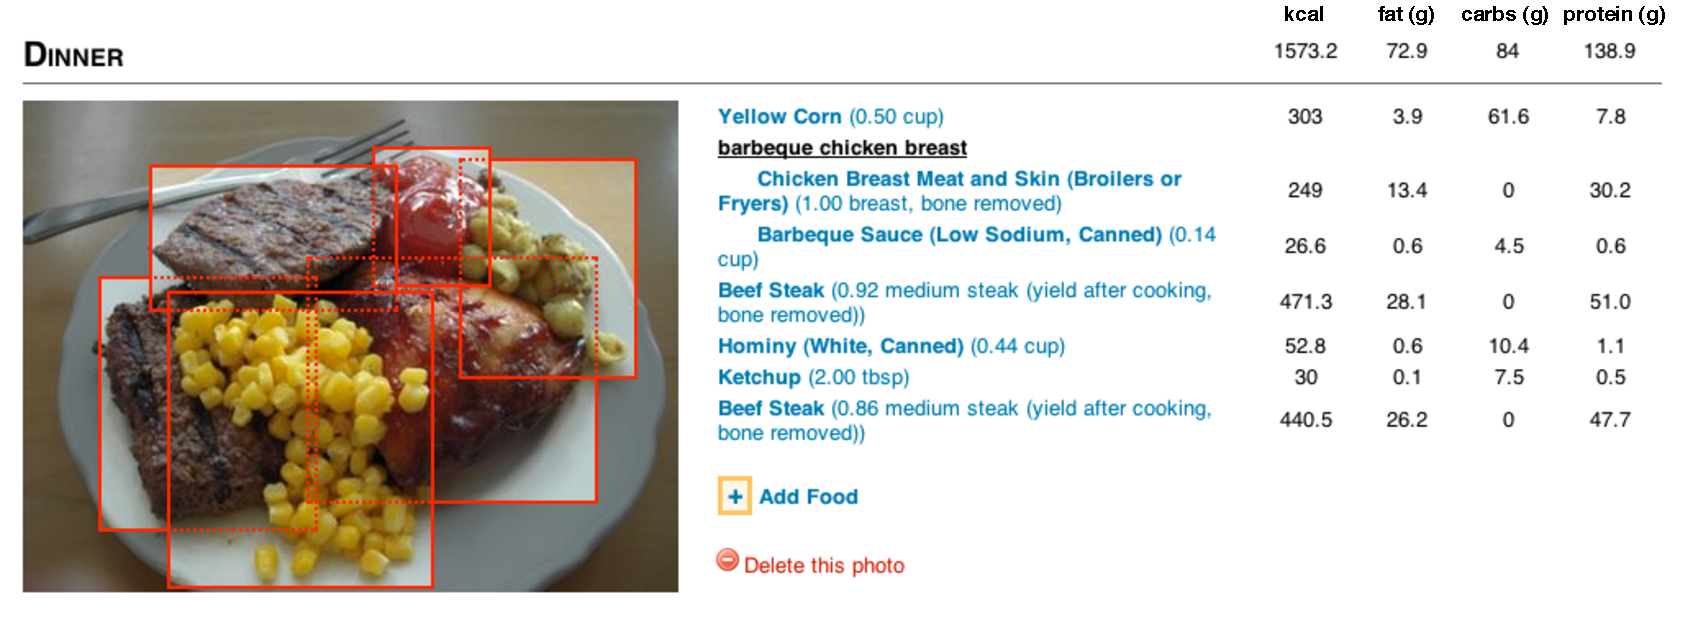
\includegraphics[width=\linewidth]{figs/ui-withHeaders.pdf}
   \caption{The PlateMate user interface.  Users upload photographs of their meals, which are processed through Mechanical Turk to produce a list of foods, serving sizes, and nutrition information.}
   \label{fig:ui}
\end{center}
\end{figure*}

\section{RELATED WORK}

%Prior work makes clear that eating depends on a variety of
%environmental and personal factors, with accurate nutritional
%information as a ``necessary but not sufficient'' condition for
%positive eating behavior
%modification~\cite{worsley2002nutrition}. Recording consumption is
%useful for dieting in particular~\cite{baker1993self}, but nutrition
%knowledge is also correlated with healthy eating more
%broadly~\cite{wardle2000nutrition}.


Nutritionists have established several methods for measuring food
intake. One prominent approach is 24-hour recall, in which a trained
dietitian interviews a subject about her consumption over the previous
day~\cite{martin2009novel}. Accuracy depends on the subject's memory
and honesty, and the technique requires a costly expert to conduct
analysis. The main alternative is food journals, in which subjects
record meals and estimate portions themselves, usually with pen and
paper.

Both methods require significant time and self-reports also suffer from limited
accuracy. A review of nine studies found error rates from $-76\%$
(underestimates) to $+24\%$
(overestimates)~\cite{schoeller1990inaccuracies}. Prior work also
suggests a dangerous bias in self-report methods. Most subjects
selectively underreport fat intake, and obese people underestimate
portions much more than leaner
ones~\cite{pikholz2004under,goris2000undereating}. These errors imply
a larger problem of self-deception, especially in vulnerable groups.

A number of online interfaces exist to simplify the process of food
logging. Smartphone applications and online calorie databases improve
on earlier methods by performing calculations automatically. However,
they still require tedious logging that discourages
recording. Self-reports using these interfaces are no more accurate
than pen and paper~\cite{ann2006use,yon2007personal}.

The Computer Science community has explored additional alternatives,
such as automatic analysis of chewing sounds~\cite{amft05:analysis}
and scanned grocery receipts~\cite{mankoff02:using}.  These methods,
while potentially more scalable and less time-consuming than current
approaches, remain inaccurate.

Martin et al. recently suggested an alternative approach called the
Remote Food Photography Method (RFPM)~\cite{martin2009novel}. Rather
than typing names of foods and estimating portions, users take photographs of their plates \newcontent{both at the beginning
  of the meal and at the end to accurately capture how much food was actually eaten.} Trained dietitians identify the pictured foods remotely
and estimate portions.  The results of laboratory studies showed that
dietitians using RFPM underestimated calories by
5-7\% compared to the ground truth obtained by directly weighing the foods~\cite{martin2009novel}.

RFPM thus combines the accuracy of direct observation by experts with the
convenience of free-living conditions. Users of the method found it
extremely satisfying and easy to use~\cite{martin2009novel}. The
problem is cost. RFPM relies on experts to analyze each
photograph, limiting the system's accessibility and potential
scale. %The method might be feasible in specific healthcare settings, but trained dietitians are too scarce for general use.

Kitamura et al. attempted to use computer vision to cheaply implement
RFPM~\cite{kitamura2010image}.  They were successful in
algorithmically detecting if a photograph contained food and in
estimating amounts of general categories of food, such as meats,
grains, and fruit.  They did not attempt to identify the specific
foods in a photo or provide actual intake totals.

The cost of experts and limitations of computer vision suggest an
opportunity for crowdsourced nutritional analysis. Prior research indicates that
the most difficult part of nutritional analysis is estimating portion
size~\cite{martin2009novel}, and that trained amateurs have low bias
but high variance~\cite{martin2007empirical}. The ``wisdom of crowds''
is ideally suited to these situations, since the average of amateur
estimates often beats a single expert~\cite{wisdom}. 
%Crowdsourcing
%using today's tools, however, creates new challenges. Workers are
%untrained, and their incentives are not the same as those of
%professional nutritionists working with a specific patient.

A recent iPhone application demonstrates, however, that naive approaches to
crowdsourcing for nutritional analysis are not sufficient. In April, 2011, the fitness
website Daily Burn released Meal Snap, which allows users to
photograph foods and receive calorie estimates by so-called ``pure
magic.''\footnote{\url{http://mealsnap.com/}, accessed July 5, 2011} Meal Snap creates
\newcontent{a single Mechanical Turk task for each image.} Workers
provide a free text description of food, and the application appears
to match this description with a database of average consumption to
estimate a range of possible calories. This approach is appealing, but
critics have accused it of failing to provide useful
data\footnote{\url{http://www.mobilecrunch.com/2011/04/05/too-lazy-to-count-calories-now-you-can-}\\\url{just-take-a-picture-of-your-meal/}} and our evaluation showed that Meal Snap's results do not correlate with the meal's actual caloric content.


\newcontent{PhotoCalorie\footnote{\url{http://photocalorie.com/},
    accessed on July 5, 2011} is a recent on-line tool that encourages
  users to upload photographs of their meals, but it uses them just to
  illustrate the user's personal photo journal.  The apparent similarity to PlateMate is superficial because to obtain calorie
  estimates, users have to enter short descriptions of the contents of
  the meals and manually estimate the amounts eaten.}

\documentclass{article}

\usepackage{times}
\usepackage{uist}
\usepackage[colorlinks=true,linkcolor=black, citecolor=black,bookmarks=true,pdfauthor={Jon Noronha, Eric Hysen, Haoqi Zhang, and Krzysztof Z. Gajos},pdftitle={PlateMate: Crowdsourcing Nutrition Analysis from Food Photographs}]{hyperref}
\usepackage{graphics}
\usepackage{graphicx}
\usepackage[usenames,dvipsnames]{color}
\usepackage{subfigure}
\usepackage{url}


\begin{document}

% --- Copyright notice ---
\conferenceinfo{UIST'11}{October 16-19, 2011, Santa Barbara, CA, USA}
\CopyrightYear{2011}
\crdata{978-1-4503-0716-1/11/10}

% Uncomment the following line to hide the copyright notice
% \toappear{}
% ------------------------

%\bibliographystyle{plain}

\title{PlateMate: Crowdsourcing Nutrition Analysis from Food Photographs}

%%
%% Note on formatting authors at different institutions, as shown below:
%% Change width arg (currently 7cm) to parbox commands as needed to
%% accommodate widest lines, taking care not to overflow the 17.8cm line width.
%% Add or delete parboxes for additional authors at different institutions. 
%% If additional authors won't fit in one row, you can add a "\\"  at the
%% end of a parbox's closing "}" to have the next parbox start a new row.
%% Be sure NOT to put any blank lines between parbox commands!
%%

\author{
\parbox[t]{12cm}{\centering
	     {\em Jon Noronha, Eric Hysen, Haoqi Zhang, Krzysztof Z. Gajos}\\
	     Harvard School of Engineering and Applied Sciences\\
	   	33 Oxford St.,
	     Cambridge, MA 02138, USA\\
	     \{noronha,hysen,hqz,kgajos\}@seas.harvard.edu}
}

%% \author{
%% \parbox[t]{9cm}{\centering
%% 	     {\em Submission 433}\\
%% 	    }
%% }

\maketitle

\newcommand{\bug}
    {\mbox{\rule{2mm}{2mm}}}
\newcommand{\Bug}[1]
    {\bug \footnote{BUG: {#1}}}
    
\newcommand{\fix}[1]{\marginpar{\centering \textcolor{Magenta}{** FIX **}}{\color{Magenta}#1}}
\newcommand{\newcontent}[1]{#1}
\newcommand{\cut}[1]{\marginpar{\centering \textcolor{Red}{CUT? **}}{\color{Red}#1}}


\abstract We introduce PlateMate, a system that allows users to take photos of their meals and
receive estimates of food intake and composition. Accurate awareness
of this information can help people monitor their progress towards  
 dieting goals, but current
methods for food logging via self-reporting, expert observation, or
algorithmic analysis are time-consuming, expensive, or inaccurate.
PlateMate crowdsources nutritional analysis from photographs using
Amazon Mechanical Turk, automatically coordinating untrained workers
to estimate a meal's calories, fat, carbohydrates, and protein.  We
present the Management framework for crowdsourcing complex tasks,
which supports PlateMate's nutrition analysis workflow. Results of our evaluations
show that PlateMate is nearly as accurate as a trained
dietitian and easier to use for most users than traditional
self-reporting.
%\fix{propose drop: ``while remaining robust for general use across a wide
%variety of meal types.'' -- especially given problem with certain types such as soups.}

\classification{H5.2 [Information interfaces and presentation]:
User Interfaces. - Graphical user interfaces.}

\terms{Design, Human Factors}

\keywords{Human computation, Crowdsourcing, Mechanical Turk, Nutrition, Remote Food Photography}

  % makes some lines with lots of white space, but 	
  % tends to prevent words from sticking out in the margin
\tolerance=4000 
% these lines help eliminate widows/orphans
\widowpenalty=10000
\clubpenalty=10000

\interfootnotelinepenalty=10000

\section{INTRODUCTION}

%Everyone wants a nutritious diet,
%\fix{[in the citation here it says that only 2 out of 10 people want to improve their diet -- so it's hard to say everyone wants a nutritious diet when this is the case..]} 
%but 
The majority of Americans perceive
healthy eating as complicated~\cite{dinkins2000beliefs}.  Seeking
comprehensible and actionable advice, Americans spend over \$40
billion each year on diets and self-help
books~\cite{reisner08:diet},
%\cite{hoffmann05:costly,reisner08:diet}, 
%\fix{[Is the first citation a Forbes.com article? I couldn't access it.]} 
but achieve little
success: the majority eventually regain any lost weight and
more~\cite{mann2007medicare}.

%Everyone wants a nutritious diet, but healthy eating is hard. New
%Years resolutions flounder while more and more miracle diets
%proliferate each year. Restaurants and grocery stores capitalize on
%these challenges with low-fat menus and healthy-choice aisles, but
%little seems to change.  Part of the problem is that people lack
%information. They have no systematic record of what they are eating
%or what it was made of. This information is not sufficient for
%healthier eating, but it seems to be a necessary
%prerequisite~\cite{worsley2002nutrition}.

There are many factors that may impact successful long-term change in
eating habits.  \newcontent{Our work is based on the observation that
  food intake monitoring is a popular component of many diets.  For
  people who make a commitment to changing their eating habits,
  accurate logs of what they eat may help in monitoring progress
  toward set goals~\cite{locke02:building}.  Currently, food logging
  is typically done by hand using paper diaries, spreadsheets, or a
  growing number of specialized applications.}  This process is both
time-consuming and
error-prone~\cite{pikholz2004under,goris2000undereating}.
Nutritionists have explored alternative methods such as daily
interviews with trained experts. While these methods improve accuracy,
they are costly and still require substantial time investment.


%There are many factors that impact successful long-term behavior
%change.  Our work is based on the observation that maintaining
%accurate awareness of nutritional intake is a prerequisite for
%changing eating
%habits~\cite{worsley2002nutrition,baker1993self}. Indeed, most diets
%require followers to track their meals, and people typically do so
%with pen and paper or computer spreadsheets.  This process is both
%time-consuming and
%error-prone~\cite{pikholz2004under,goris2000undereating}.
%Nutritionists have explored alternative methods such as daily
%interviews with trained experts. These methods improve accuracy, but
%they are costly and still require substantial time investment.

Our work is inspired by the \emph{Remote Food Photography Method} (RFPM)~\cite{martin2009novel}, a novel approach from the nutrition literature. Rather
than remembering foods or writing down records, users take
\newcontent{two photographs of each meal: one at the beginning
  of the meal and one at the end documenting the leftovers.}
These images are analyzed by a third party, making logging easier and
discouraging self-deception. The challenge is in finding a qualified
third party without prohibitive costs. Expert nutritionists are 
scarce and costly, limiting the system to wealthy users or patients with
particular conditions.

To make accurate food logging easier and more affordable, we introduce
\emph{PlateMate}, a system for crowdsourcing nutritional analysis
(calories, fat, carbohydrates, and protein) from photographs of meals
using Amazon Mechanical Turk.
%PlateMate automatically coordinates untrained workers to estimate a meal's calories, fat, carbohydrates, and protein from a photograph. 
Complex tasks like this are hard problems for
crowdsourcing, as workers may vary drastically in experience and
reliability. To achieve accurate estimates, we propose a workflow in 
which the overall problem is decomposed into
small, manageable, and verifiable steps.
%\fix{perhaps note right here that we focus on estimating nutritional information under the assumption that the user eats what he or she photographs, and leave handling leftovers for future work? If do so here then drop next sentence maybe.} 
PlateMate uses this workflow to assign tasks to contributors, to validate and combine results, and to appropriately route tasks for further processing.
%\fix{tried to edit the text here some to be more specific as to what is assigned, validated, combined, routed --- some more specificity may help even more}
%Tasks are assigned,
%validated, combined, and appropriately routed through a larger
%workflow.

This paper makes three main contributions:
%\vspace*{-2mm}
\begin{enumerate}
\item We present PlateMate, an end-to-end system for crowdsourced nutrition analysis from food photographs.
\item We discuss the results of a two-part evaluation, which suggests
  PlateMate can be as accurate as experts and self-report methods, and
  more usable than manual logging for everyday use.
\newcontent{\item We introduce the Management framework---inspired by the structure of human organizations, it provides effective support for managing crowdsourcing of complex heterogeneous tasks.  }
% by coordinating contributions using a hierarchical message-passing system.}
\end{enumerate}
%\vspace*{-2mm}

%PlateMate implements the first of the two steps of the Remote Food
%Photography Method, that is, it performs nutrition analysis based on
%measurements of photographs of original portions. While the system can
%also be used on photographs of leftovers, other approaches that employ
%information obtained from measuring original portions in the process
%of measuring leftovers are possible and may actually be more efficient
%for the second step. In some situations, the second step may involve
%additional challenges, e.g., as caused by messy leftover plates where
%foods lose their original textual and shape and may thus be hard to
%identify.  Given that the first step is necessary for the RFPM method
%and that results from evaluating PlateMate will provide useful lessons
%for designing for the second step, for simplicity we focus on
%measuring original portions and leave handling of food waste for
%future work.

PlateMate implements the first step in the Remote Food Photography Method.  In the last section we suggest how it can be extended to also support the second step: the analysis of photographs of food waste.
 
In the next section we review relevant prior work.  We then describe
the design and implementation of the PlateMate system and its
components. Next, we discuss our Management framework.
We then present an evaluation of the accuracy and usability of
PlateMate and discuss the results. Finally, we consider future
extensions to PlateMate.

\begin{figure*}[t]
\begin{center}
   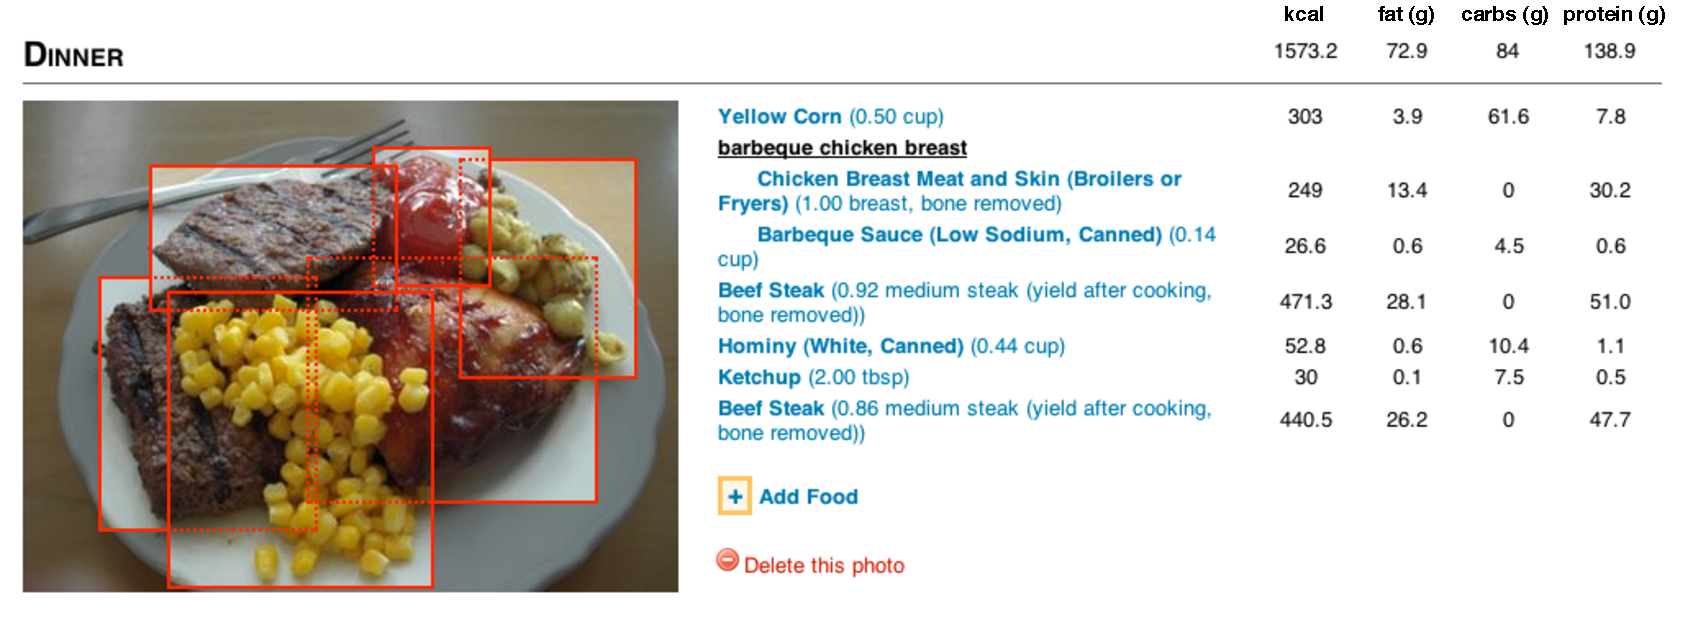
\includegraphics[width=\linewidth]{figs/ui-withHeaders.pdf}
   \caption{The PlateMate user interface.  Users upload photographs of their meals, which are processed through Mechanical Turk to produce a list of foods, serving sizes, and nutrition information.}
   \label{fig:ui}
\end{center}
\end{figure*}

\section{RELATED WORK}

%Prior work makes clear that eating depends on a variety of
%environmental and personal factors, with accurate nutritional
%information as a ``necessary but not sufficient'' condition for
%positive eating behavior
%modification~\cite{worsley2002nutrition}. Recording consumption is
%useful for dieting in particular~\cite{baker1993self}, but nutrition
%knowledge is also correlated with healthy eating more
%broadly~\cite{wardle2000nutrition}.


Nutritionists have established several methods for measuring food
intake. One prominent approach is 24-hour recall, in which a trained
dietitian interviews a subject about her consumption over the previous
day~\cite{martin2009novel}. Accuracy depends on the subject's memory
and honesty, and the technique requires a costly expert to conduct
analysis. The main alternative is food journals, in which subjects
record meals and estimate portions themselves, usually with pen and
paper.

Both methods require significant time and self-reports also suffer from limited
accuracy. A review of nine studies found error rates from $-76\%$
(underestimates) to $+24\%$
(overestimates)~\cite{schoeller1990inaccuracies}. Prior work also
suggests a dangerous bias in self-report methods. Most subjects
selectively underreport fat intake, and obese people underestimate
portions much more than leaner
ones~\cite{pikholz2004under,goris2000undereating}. These errors imply
a larger problem of self-deception, especially in vulnerable groups.

A number of online interfaces exist to simplify the process of food
logging. Smartphone applications and online calorie databases improve
on earlier methods by performing calculations automatically. However,
they still require tedious logging that discourages
recording. Self-reports using these interfaces are no more accurate
than pen and paper~\cite{ann2006use,yon2007personal}.

The Computer Science community has explored additional alternatives,
such as automatic analysis of chewing sounds~\cite{amft05:analysis}
and scanned grocery receipts~\cite{mankoff02:using}.  These methods,
while potentially more scalable and less time-consuming than current
approaches, remain inaccurate.

Martin et al. recently suggested an alternative approach called the
Remote Food Photography Method (RFPM)~\cite{martin2009novel}. Rather
than typing names of foods and estimating portions, users take photographs of their plates \newcontent{both at the beginning
  of the meal and at the end to accurately capture how much food was actually eaten.} Trained dietitians identify the pictured foods remotely
and estimate portions.  The results of laboratory studies showed that
dietitians using RFPM underestimated calories by
5-7\% compared to the ground truth obtained by directly weighing the foods~\cite{martin2009novel}.

RFPM thus combines the accuracy of direct observation by experts with the
convenience of free-living conditions. Users of the method found it
extremely satisfying and easy to use~\cite{martin2009novel}. The
problem is cost. RFPM relies on experts to analyze each
photograph, limiting the system's accessibility and potential
scale. %The method might be feasible in specific healthcare settings, but trained dietitians are too scarce for general use.

Kitamura et al. attempted to use computer vision to cheaply implement
RFPM~\cite{kitamura2010image}.  They were successful in
algorithmically detecting if a photograph contained food and in
estimating amounts of general categories of food, such as meats,
grains, and fruit.  They did not attempt to identify the specific
foods in a photo or provide actual intake totals.

The cost of experts and limitations of computer vision suggest an
opportunity for crowdsourced nutritional analysis. Prior research indicates that
the most difficult part of nutritional analysis is estimating portion
size~\cite{martin2009novel}, and that trained amateurs have low bias
but high variance~\cite{martin2007empirical}. The ``wisdom of crowds''
is ideally suited to these situations, since the average of amateur
estimates often beats a single expert~\cite{wisdom}. 
%Crowdsourcing
%using today's tools, however, creates new challenges. Workers are
%untrained, and their incentives are not the same as those of
%professional nutritionists working with a specific patient.

A recent iPhone application demonstrates, however, that naive approaches to
crowdsourcing for nutritional analysis are not sufficient. In April, 2011, the fitness
website Daily Burn released Meal Snap, which allows users to
photograph foods and receive calorie estimates by so-called ``pure
magic.''\footnote{\url{http://mealsnap.com/}, accessed July 5, 2011} Meal Snap creates
\newcontent{a single Mechanical Turk task for each image.} Workers
provide a free text description of food, and the application appears
to match this description with a database of average consumption to
estimate a range of possible calories. This approach is appealing, but
critics have accused it of failing to provide useful
data\footnote{\url{http://www.mobilecrunch.com/2011/04/05/too-lazy-to-count-calories-now-you-can-}\\\url{just-take-a-picture-of-your-meal/}} and our evaluation showed that Meal Snap's results do not correlate with the meal's actual caloric content.


\newcontent{PhotoCalorie\footnote{\url{http://photocalorie.com/},
    accessed on July 5, 2011} is a recent on-line tool that encourages
  users to upload photographs of their meals, but it uses them just to
  illustrate the user's personal photo journal.  The apparent similarity to PlateMate is superficial because to obtain calorie
  estimates, users have to enter short descriptions of the contents of
  the meals and manually estimate the amounts eaten.}

\documentclass{article}

\usepackage{times}
\usepackage{uist}
\usepackage[colorlinks=true,linkcolor=black, citecolor=black,bookmarks=true,pdfauthor={Jon Noronha, Eric Hysen, Haoqi Zhang, and Krzysztof Z. Gajos},pdftitle={PlateMate: Crowdsourcing Nutrition Analysis from Food Photographs}]{hyperref}
\usepackage{graphics}
\usepackage{graphicx}
\usepackage[usenames,dvipsnames]{color}
\usepackage{subfigure}
\usepackage{url}


\begin{document}

% --- Copyright notice ---
\conferenceinfo{UIST'11}{October 16-19, 2011, Santa Barbara, CA, USA}
\CopyrightYear{2011}
\crdata{978-1-4503-0716-1/11/10}

% Uncomment the following line to hide the copyright notice
% \toappear{}
% ------------------------

%\bibliographystyle{plain}

\title{PlateMate: Crowdsourcing Nutrition Analysis from Food Photographs}

%%
%% Note on formatting authors at different institutions, as shown below:
%% Change width arg (currently 7cm) to parbox commands as needed to
%% accommodate widest lines, taking care not to overflow the 17.8cm line width.
%% Add or delete parboxes for additional authors at different institutions. 
%% If additional authors won't fit in one row, you can add a "\\"  at the
%% end of a parbox's closing "}" to have the next parbox start a new row.
%% Be sure NOT to put any blank lines between parbox commands!
%%

\author{
\parbox[t]{12cm}{\centering
	     {\em Jon Noronha, Eric Hysen, Haoqi Zhang, Krzysztof Z. Gajos}\\
	     Harvard School of Engineering and Applied Sciences\\
	   	33 Oxford St.,
	     Cambridge, MA 02138, USA\\
	     \{noronha,hysen,hqz,kgajos\}@seas.harvard.edu}
}

%% \author{
%% \parbox[t]{9cm}{\centering
%% 	     {\em Submission 433}\\
%% 	    }
%% }

\maketitle

\input{macros}

\abstract We introduce PlateMate, a system that allows users to take photos of their meals and
receive estimates of food intake and composition. Accurate awareness
of this information can help people monitor their progress towards  
 dieting goals, but current
methods for food logging via self-reporting, expert observation, or
algorithmic analysis are time-consuming, expensive, or inaccurate.
PlateMate crowdsources nutritional analysis from photographs using
Amazon Mechanical Turk, automatically coordinating untrained workers
to estimate a meal's calories, fat, carbohydrates, and protein.  We
present the Management framework for crowdsourcing complex tasks,
which supports PlateMate's nutrition analysis workflow. Results of our evaluations
show that PlateMate is nearly as accurate as a trained
dietitian and easier to use for most users than traditional
self-reporting.
%\fix{propose drop: ``while remaining robust for general use across a wide
%variety of meal types.'' -- especially given problem with certain types such as soups.}

\classification{H5.2 [Information interfaces and presentation]:
User Interfaces. - Graphical user interfaces.}

\terms{Design, Human Factors}

\keywords{Human computation, Crowdsourcing, Mechanical Turk, Nutrition, Remote Food Photography}

  % makes some lines with lots of white space, but 	
  % tends to prevent words from sticking out in the margin
\tolerance=4000 
% these lines help eliminate widows/orphans
\widowpenalty=10000
\clubpenalty=10000

\interfootnotelinepenalty=10000

\input{sections/intro}
\input{sections/relatedwork}
\input{sections/platemate}
\input{sections/management}
\input{sections/evaluation}
\input{sections/discussion}
\input{sections/conclusion}



% bibliography --- please add new references to the platemate.bib
%\small % a little space saving device
\begin{flushleft}
\bibliographystyle{unm}
\bibliography{platemate,kzg}
\end{flushleft}

\end{document}

\section{THE MANAGEMENT FRAMEWORK}
In this section, we introduce a programming framework for solving
problems with crowds based on a human organizational hierarchy. This
approach differs conceptually from prior work, which has focused on
creating ``crowd programming languages'' that combine human and
machine computation. For example, TurKit~\cite{little2010turkit} lets requesters
program crowds in JavaScript, Qurk~\cite{qurk} integrated crowds into
SQL, and CrowdForge~\cite{crowdforge} parallelized work with MapReduce
scripts. In each case, these toolkits have attempted to make working
with crowds more like working with computers.
This approach emphasizes computation as the natural glue for combining individual worker contributions and the resulting artifact is a computer program with some of the primitive operations implemented as ``functional calls'' to human workers~\cite{little2010turkit}.

Because PlateMate relies primarily on human work, divided into a number of heterogenous and interacting tasks, and because the issues of worker skill and motivation were central to our design process, we found it conceptually helpful to use human organizational hierarchies as the metaphor for designing our system.  Specifically, we observe that in the real world, expert-level work (e.g., building a table) can be reproduced by less skilled workers---each working on a specific part of the process---supervised by managers who are not necessarily skilled craftsmen themselves, but who know how to assign tasks, route work among workers, and verify the quality of the work.

%To illustrate, in the real world, expert-level work can be reproduced by less skilled workers
%through division of labor in an organized hierarchy. Large, complex
%goals are decomposed into simpler operations overseen by managers who
%supervise workers with clear areas of responsibility. Consider making
%a table. One approach is to have a highly-trained expert craftsman
%build the table alone. Alternatively, a factory can build a table by
%assigning each worker a small piece of the job. One worker may saw
%the wood, another may polish it, and a third may assemble the
%pieces together. Supervisors---who need not be experts, either---assign tasks to workers, route work between them, and verify the quality of work. 

%Such approach is conceptually useful for processing large computational tasks with human
%intelligence as an extra ``functional call''~\cite{little2010turkit}. 

%PlateMate,
%however, aims to emulate the reasoning of an individual human
%expert. In this domain, we found the abstraction of ``programming
%crowds'' as if they were computers unnatural. 
%We could not think of
%the crowd as a function call, since our HITs and workflows were based
%on careful observation of Turker psychology and motivation. 
%Instead, 
%PlateMate
%thus follows the opposite approach. 

%With PlateMate, however, we 
%
%PlateMate tries to make programming crowds more like instructing and
%organizing a team of humans.


%This approach of distributing
%work has been profoundly successful with material goods, and we seek
%to do the same thing with expert thought and reasoning.\fix{Consider removing this last sentence -- this is a broad claim with no citations.}



%\section{The Management Framework}
Thus, to implement division of labor for crowdsourcing, we created a new
framework organized around objects called \em managers.\em\  
%Managers are independent of their peers.  
%written as if they are independent agents in a distributed system. 
Managers communicate with their supervisors and their \em employees \em using asynchronous message passing: managers assign tasks by placing them in inboxes of lower level managers and communicate with their superiors by placing results of completed tasks in their own outboxes.
%They constantly check for new assignments, assign work to
%their \em employees,\em\ receive completed work, and send their own outputs up
%the hierarchy. 
This hierarchical message-passing approach allows programmers
to implement workflows by decomposing problems into progressively
smaller steps.

As illustrated earlier in Figure~\ref{fig:system}, the root of this tree is a \em chief \em manager, which gathers new inputs
and produces completed outputs. In PlateMate, the chief has three
employees: Tag, Identify, and Measure. Each of these are in turn
managers and have their own employees, corresponding to the individual
HITs described above.

This hierarchical structure creates a flexible workflow consisting of
 modules connected by higher-level managers. Managers can route work intelligently among their
employees, and may dynamically alter the sequence of steps in the process depending on a situation. For example, PlateMate's Tag manager compares the outputs from its
DrawBoxes employee. If they are sufficiently different, they are sent
to the VoteBoxes manager to decide between them. Otherwise, one answer
is chosen randomly and sent up the hierarchy as Tag's completed
output. All managers work in parallel, each processing its own stream of
work. 

When multiple tasks are submitted, processing is done just-in-time: for example, as soon as one photograph is tagged, the Identify manager begins the process of finding out what foods are present in each of the boxes without waiting for the remaining photographs to be tagged.  

%This asynchronous approach improves on the iterative workflows
%in TurKit, where each stage blocks until every task in that stage has
%been completed. 
%It also differs from CrowdForge, where intermediate
%outputs must all be finished before they can be recombined. Instead,
%completed work is sent up the chain and on to the next step
%immediately, where another manager can begin to process it.

At the lowest level of the hierarchy are managers whose employees are
the crowd workers. Managers at this level create jobs (such as asking
for the food in one tagged box on a photo to be identified) and
receive responses. Programmers create HIT templates and validation
functions which are used by the framework to create HITs and approve
work. Managers simply assign work to the crowd and receive validated outputs that can be passed up the
tree.

Of course, the Management Framework \em is \em a computational framework, and it naturally supports a number of the recently introduced design patterns for programming the crowds.  For example, the Tag step is an analog of the map step in MapReduce and the Describe step (part of Identify, see Figure~\ref{fig:system}) relies on iterative refinement~\cite{little10:exploring} to improve the level of detail of the descriptions.

Management is implemented as an extension of Django, a web application
framework for Python. It builds on several useful features from
Django, including an HTML template language for defining HIT
instructions, examples, and interfaces. It also uses Django's
object-relational mapper, which automatically stores Python objects in
a MySQL database. This means that the precise state of the system is
always stored, including managers' inboxes and outboxes, active HITs
and completed assignments, and intermediate inputs and outputs. This
simplifies later analysis, since requesters can go back and query
responses from each stage in the workflow. It also protects completed
work from program errors or service outages; after crashes, execution simply  
resumes from the last good state. 
%\fix{drop this: ``rather than restarting from the
%beginning as in TurKit's crash-and-rerun
%model~\cite{little2010turkit}.'' -- turkit doesn't really start from the beginning, it also picks up where 
%you leave off}



\section{EVALUATION}

Our evaluation focused on PlateMate's feasibility as a replacement for traditional food logging.  We considered three broad criteria:
\vspace*{-2mm}
\begin{enumerate}
\item \textbf{Accuracy.} How accurate were crowdsourced estimates compared to current alternatives? Could users trust them?
\item \textbf{Usability.} How much effort or discomfort would users experience in photographing food, uploading the photos, and correcting errors in PlateMate's estimates?
\item \textbf{Robustness.} How well does the PlateMate system fare with ``real world'' photographs?
\end{enumerate}
\vspace*{-2mm}
We designed two experiments to answer these questions.  In the first, nutrition data returned from PlateMate was compared with ground truth, expert dietitian estimates, and a recent commercial application.  In the second study, ten participants used PlateMate and a manual food-logging system for four days.

\subsection{Evaluation of Accuracy}

Our first study had two goals. The first was to determine the accuracy of PlateMate with ground truth data obtained from manufacturers or preparers. The second was to compare PlateMate's performance with two alternative approaches to remote food photography: analysis by experts and results from Meal Snap.  
\newcontent{Because Meal Snap only returns calorie information and to make the task manageable for our expert participants, we limited our comparison to estimated calories even though PlateMate generates reports that also include fat, protein, and carbohydrates.}

\begin{figure}
\begin{center}
   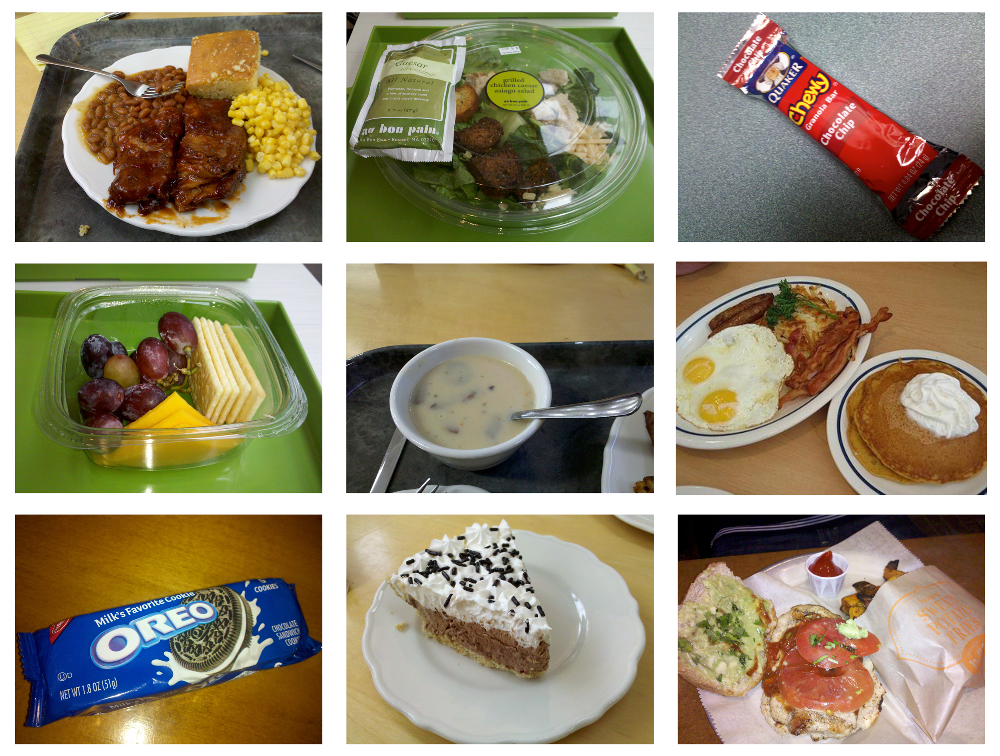
\includegraphics[width=\columnwidth]{figs/groundtruth.pdf}
   \caption{Examples of photos from the study of PlateMate's accuracy.}
   \label{fig:groundTruth}
\end{center}
\end{figure}

\subsubsection{Method}
We conducted the experiment with a sample of 18 photographs showing 36 distinct foods. Some depicted individual foods or packages, while others showed complex plates containing many items, as shown in Figure~\ref{fig:groundTruth}.  Each pictured food had nutritional data available through the manufacturer or preparer, and foods were weighed when necessary to ensure accuracy. These foods were selected to span a variety of meals and sources, including restaurants, cafeterias, and grocery items.  We also included a mix of simple foods and composite items like salads and sandwiches.

We recruited three professional dietitians to provide expert estimates: one was a private nutrition counselor, and the other two were employed by a hospital. They received compensation for their time and provided estimates from their own offices. They were encouraged to use any aids, like books and calorie databases, that they would typically use for a similar task.
% Note that their analysis is not directly comparable to the expert estimates in the original RFPM study~\cite{martin2009novel}. That experiment focused only on measuring portions, and experts were told what the foods were and provided with photographs of standard portions of each. Our study focused on genuine remote analysis, where experts had only the picture to work from. 

Our third set of estimates came from Meal Snap, a recent commercial application.  Meal Snap returns a range of calories rather than a definitive answer, so we used the mean of its high and low values.  

\begin{figure}
\begin{center}
   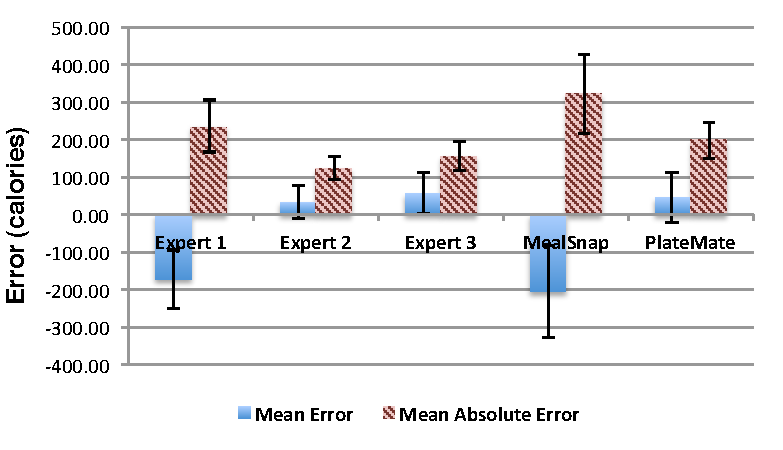
\includegraphics[width=\columnwidth]{figs/error-both}
   \caption{Mean errors (i.e., overall bias) and mean absolute errors (average magnitude of an error) for estimates made by the human experts, the Meal Snap application, and PlateMate compared to data provided by manufacturer or preparer.  Error bars correspond to standard error.}
   \label{fig:error}
\end{center}
\end{figure}

\subsubsection{Results}

In terms of mean absolute error on calorie estimates, PlateMate was not significantly different from the human experts or the Meal Snap application.  Figure~\ref{fig:error} illustrates the results in detail.  
As expected, trained dietitians were the most accurate on average. Their mean absolute error rates were $39.4\%$, $20.8\%$, and $26.1\%$, for an average of $172.0$ calories or $28.7\%$ per photograph. The best expert was off by just $124.5$ calories, on average. PlateMate was close behind with a mean absolute error rate of $198$ calories, or $33.2\%$.  MealSnap was farther behind, with an average error rate of $322.8$ calories or $53.9\%$.

Absolute error rates reflect the average magnitude of the error, but not the biases in each method. To understand how estimates from each source would add up over time, we also measured mean error without taking absolute values. The best expert overestimated by just 32.75 calories on average, for a mean error rate of $+5.5\%$.  The other two experts had error rates of $+9.2\%$ and $-27.5\%$.

%This result was in line with~\cite{martin2009novel}, which found trained nutritionists underestimated portions with an error rate of $-6.6\%$, though our task also required identifying the foods.

In comparison, PlateMate had a mean error rate of $+44.1$ calories, or $+7.4\%$, which was much closer than Meal Snap's $-34.4\%$. Expert and PlateMate results are significantly correlated with the ground truth data ($r^2 = .8626$, $.9062$, and $.9378$ for the experts, and $r^2=.8622$ for PlateMate, all with $p<.0001$), while Meal Snap results were not correlated with the actual nutritional content of the meals ($r^2=.2352$, $p=.3475$).
%MealSnap results appear almost completely uncorrelated with ground truth ($r^2=0.23$), while PlateMate and expert results were strongly correlated with actual calorie content of each food ($r^2=0.86$ and $0.93$, respectively). \bug[the $r^2$ for expert results, is this an average of the three experts?  Perhaps the better thing would be to show all three?]

%These results suggest that, while all three methods of remote food photography are somewhat inaccurate, PlateMate and experts are much better than MealSnap. MealSnap's results were almost random, while PlateMate and expert results tracked ground truth closely. PlateMate was less accurate than the best expert, but about the same as the mean.

PlateMate's error rate compares favorably to amateur self-reports, where error rates can be greater than $400$ calories/day and range from $-76\%$ to $+24\%$~\cite{schoeller1990inaccuracies,champagne2002energy}.  It also lacks the systematic bias towards underestimation in self-reports, especially among vulnerable users. These results indicate that PlateMate's answers, while imperfect, can be a useful nutritional guide.

\subsubsection{Error Analysis}

Most errors in the study corresponded to single failures in specific parts of the pipeline.   In the Tag stage, boxes were sometimes drawn improperly, leading to missing or duplicate identifications.  In one photo of a brownie and banana on a small plate, only one box was drawn covering the entire banana and most of the brownie.  As a result, the workers at the Identify stage omitted the brownie.  On a photo of a hamburger with mushrooms, overlapping boxes were drawn over the burger and topping.  In this case, the mushrooms were identified in both boxes.  

Most errors occurred in the Identify stage.  Turkers had trouble distinguishing similar types of a food, which sometimes had large nutrition differences.  A plate of vegetarian baked beans was identified as regular baked beans, tripling the calorie count.  Branded foods also caused problems: a relatively low-calorie chicken sandwich was identified as a sandwich from the restaurant Chili's, which had over twice as many calories.  Another common situation involved duplication with both a composite item and one or more foods included in that composite both being selected.  A slice of pizza with pepperoni and olives was identified as ``Pizza with Meat and Vegetables,'' ``Pepperoni,'' and ``Black Olives,'' duplicating the toppings.

During measurement, many very small quantities were overestimated, especially when a small amount of a food was spread over a large area.  A dash of parsley on a sandwich was overestimated as .27 cups, for example.  Other errors occurred when one food appeared in several boxes. This led to a hamburger bun being counted as two buns when each half of the bun was seen in its own box.

\subsection{User Study}
Our second study looked at the subjective experience of using PlateMate as an end-to-end system for nutritional monitoring, compared to manual logging.  We looked for insights about the system's usability, in terms of the inconvenience of taking photographs and the effort required to correct errors.  Finally, we wanted to observe how robustly PlateMate functioned in the ``real world,'' without any constraints on the types of photographs submitted to the system.

\subsubsection{Method}
We recruited 10 participants (4 male, 6 female) via advertisements posted on several university email lists.  Seven of the participants were undergraduates, two were graduate students, and one was a faculty member.

To help us evaluate the quality of the nutritional estimates generated by PlateMate and by the participants in this study, we recruited four dietitians employed at a local hospital.  Two of them had also participated in the experiment evaluating the accuracy of PlateMate, where they produced the most accurate results. Participants and dietitians were compensated for their time.

Users were interviewed before and after the experiment. In the first interview, we discussed prior experiences tracking meals and trained participants on using the system. In the exit interview, we discussed their experiences using both logging methods.  

During the study, we asked the participants to take photographs of their meals for four days and upload them to PlateMate once a day.  For two of the days, participants received estimates generated by PlateMate and could correct those estimates.  For the other two days, participants were not shown estimates and manually logged their food.  Half of the participants used the manual system first and half used PlateMate first.  We designed the interface for manual logging and correcting estimates to resemble existing commercial tools for manual food logging.

In order to assess the results produced by PlateMate compared to current consumer best practices, we used PlateMate to generate hidden estimates for participants' photos from the two days of manual recording.  Participants only saw this data during the exit interviews, when they were asked to compare their own logging with the automatic estimates.

\begin{figure}
\begin{center}
   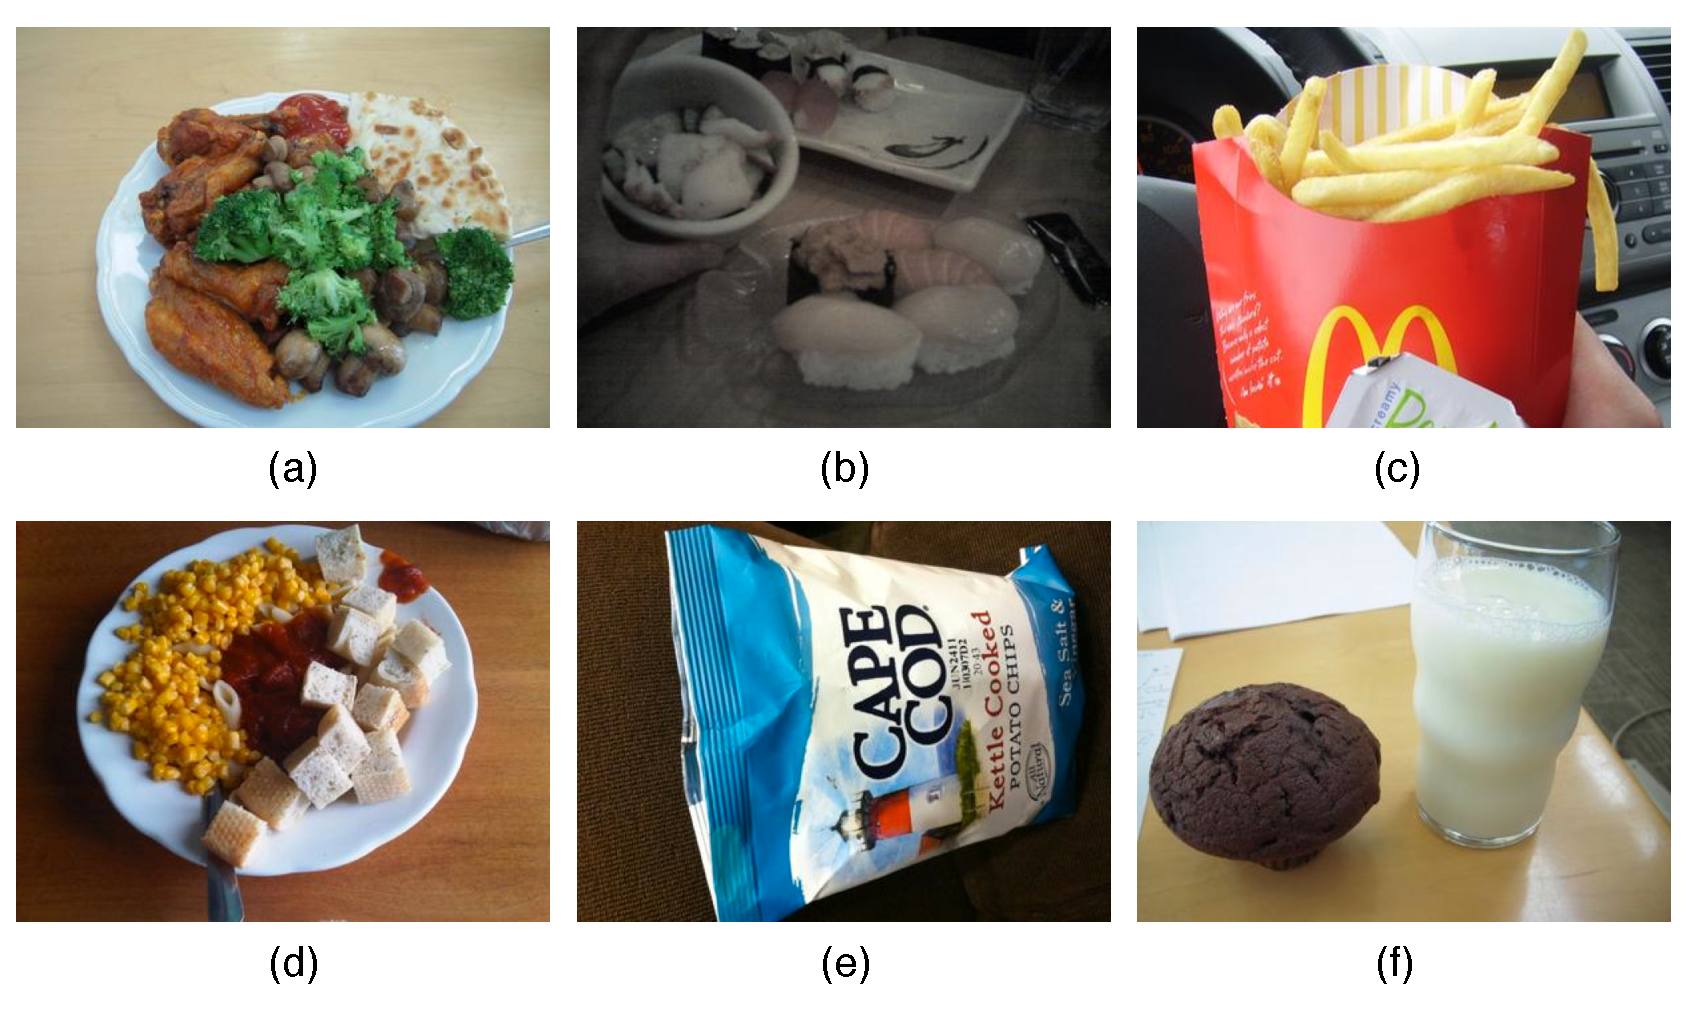
\includegraphics[width=\columnwidth]{figs/userphotos.pdf}
   \caption{Example user photos.  PlateMate handled (a) - (c) well, while (d) - (f) caused problems.  In (d) the pasta with sauce in the middle was hard to see; in (e) there is no sense of scale to determine the size of the bag; and in (f) the type of milk is unclear.}
   \label{fig:userPhotos}
\end{center}
\end{figure}

\subsubsection{Findings from the Initial Interviews}
Our pre-interviews with participants confirmed that existing methods of logging food are cumbersome. All but one of the 10 had tried logging their food at some point, but most gave up after a few days or weeks. Only two participants still tried, and neither reported doing so consistently or reliably. They recalled their attempts to keep track of food as ``annoying,'' ``inconvenient,'' and ``tedious.'' One subject recalled six separate failed attempts, each lasting just a few days. Some reported success when they were required to log for athletics or class projects, but recording lapsed when those commitments ended.

Despite these challenges, participants found nutritional information valuable. Eight participants reported looking at nutrition labels on packaged foods. Several reported looking up new foods out of curiosity. One participant reported revelations like ``Oh wow, that's a lot of calories in dressing,'' and another now dilutes her juice with water after discovering how much sugar it contains.

% I think this paragraph and the next can be cut. --EH
%Subjects acknowledged that finding this information is more difficult when foods are not packaged with labels. When eating prepared meals, especially in restaurants, they sometimes guessed crude nutrition estimates. Many had some background nutrition knowledge, which gave them a rough idea of the protein, fat, and carbohydrate levels of different kinds of foods. %One subject explained, ``When I'm at Subway getting a sandwich, I know if I get turkey and no cheese and a vinaigrette, it's better than getting the works because there's less fat.''

%Others relied on heuristics or rules of thumb for healthy eating, which don't require any systematic knowledge. Two subjects spoke of color variety and drawing from different food groups, emphasizing ``greens'' on the plate. Another spoke of eating ``like mom taught you.'' Others learned from their feelings after eating. One subject explained, ``I feel more grossed out at the fast food spots.''

\subsubsection{Exit Interview Reactions}
We asked all ten participants their preference between using PlateMate for automatic estimates and logging manually (by any method). Seven participants said they would prefer using PlateMate in the future, citing its ease of use and the convenience of ``having someone else do that for me rather than guess myself.'' One subject explained, ``My answers were closer to guesswork; this felt more like science.'' The three subjects who did not prefer PlateMate felt that they could not trust it or that the process of taking photos and correcting the estimates was too cumbersome.

Subjects were divided in their perceptions of PlateMate's
accuracy. Seven of 10 found the answers at least as good as their
own and of these four found PlateMate's estimates to be more accurate than self
reports.  After seeing his
own estimates and PlateMate's for the same meals, one subject said the
exercise ``confirmed my suspicions that you guys were more accurate
than I was. The tendency is always to say `oh, I didn't have that
much.''' Three others found their own estimates and PlateMate's
basically equivalent.

The other three subjects all found PlateMate less accurate than their
own estimates. One said that PlateMate's answers were close, ``like
$80$-$90\%$, but not perfect. I want to be sure.'' Another still
preferred PlateMate even though she could not fully trust its
results. She explained, ``For some people if it's not perfect they'll
never use it. But for me it was great...Even if it is only half of
them correct, that is fewer I have to enter manually, and the happier
I am.'' Another user disagreed, feeling that it took more effort to
correct PlateMate estimates than ``do it right myself the first
time.''

In total, seven users said that PlateMate required less effort than
manual logging, which most of these users considered unpleasant and
tedious. They called it ``annoying'', ``boring,'' and ``not
excruciating but not insignificant either.'' These participants said
PlateMate was ``definitely easier'' and ``much simpler,'' concluding
that it ``definitely saves me time and effort.'' They also found
receiving the results exciting. One user explained, ``it was more
fun...I got the email, and my friend was like, `Oh! Do we get to see
it now?''' Another was discouraged by the difficulty of manually
estimating portions, so she found it ``really helpful to have someone
else do that for me rather than guess myself.''

\subsubsection {PlateMate Performance}

Next, we analyze PlateMate's performance on photographs collected by
our users.  We wanted to investigate the system's robustness given a
broad variety of meals and realistic variations in photograph quality.
Ideally, the PlateMate estimates and manual logging data from the user
study could be compared to ground truth to determine accuracy, but
such data were clearly not available.

Instead, we first looked at the differences between participant and PlateMate estimates.  Comparing results from $112$ photos for which we had both participant and PlateMate estimates, we found the two sets of results to be positively correlated ($r^2=0.62$, $p<.0001$). PlateMate's estimates were slightly higher than participants', with a mean difference of $+41.0$ calories (median $+18.8$) or $+11.5\%$ that was not statistically significant (Wilcoxon $z=686$, {\it n.s.}). 

To gain further insight into relative accuracies of PlateMate and our participants, we presented 50 of these photographs together with both sets of nutritional estimates to 4 professional nutritionists.  The nutritionists worked in pairs.  Each pair was presented with a photo and two sets of numbers representing total calories, protein, fat, and carbohydrates.  One of these sets came from a participant and one from PlateMate, and the experts were blind to the source of the data.  They were then asked to pick the more accurate set, taking as much time as necessary and using any necessary tools and references.  The dietitians in each pair were allowed to talk to each other and could choose to agree on one data set as more accurate, disagree, or say they were unable to pick one data set as more accurate.  

%To verify the reliability of using human experts for this task, interspersed with the 50 photos from the user study were 10 photos from the ground truth study with one data set for the ground truth nutrition data and one an arbitrary error between 20\% and 50\% off of ground truth (the errors included both under- and overestimates).  Unfortunately, of the 10 ground truth photos, both pairs of dietitians picked the correct ground truth data set 50\% of the time, and we observed no bias toward either over- or underestimates.

Of the 50 user study photos, the first pair could not decide which set of nutritional estimates was more accurate in 5 cases and the second pair could not in 12 cases.  Out of the decisive photos, PlateMate data was selected as more accurate $44.4\%$ and $47.4\%$ of the time by the two pairs. These results suggest that neither method was obviously more accurate, especially since nearly half ($49.2\%$) of photos had estimates within 100 calories of each other.

% Do we need this paragraph? We're undecided. - JN
When disagreements did happen, PlateMate's estimates were larger $63.5\%$ of the time. This is consistent with our finding in the first study that PlateMate slightly overestimates and prior research that suggests a strong bias in manual recording towards underestimation.~\cite{pikholz2004under,goris2000undereating}.  PlateMate's estimates for daily energy intake were $+229.8$ calories higher than self-reports on average, a difference equivalent to four Oreo cookies every day.

\subsubsection{Error Analysis}
Many of the errors seen from the user study results were similar to those already discussed from the ground truth study, but some new issues emerged.  In measurement, we saw difficulty estimating portions when extreme close-up photos were taken with no sense of scale.  Turkers could not agree if a bag of potato chips (Figure~\ref{fig:userPhotos}) was a portion or large bag.  Scale was also a problem in identification: a small tangerine was identified as a larger orange.  Other identification errors occurred when foods with nearly correct names but vastly different nutrition were selected, like ``grapefruit juice'' and ``juice concentrate,'' which has eight times the calories. One Subway chicken sandwich was identified as ``Subway Roasted Chicken Patty,'' which could be interpreted as the whole sandwich but in fact just contained the chicken.

Human errors during manual logging mostly occurred when participants forgot to log a certain food.  In photo (f) of Figure~\ref{fig:userPhotos} the participant only recorded the milk and forgot to log the muffin, which represented most of the photo's calories.  In a photo of french fries, a participant forgot to record the dipping sauce next to the fries.  Similar errors occurred when participants sought to simplify their recordings to save time.  One subject ate a bowl of several types of fruit but recorded the entire bowl as raspberries, while PlateMate correctly identified each fruit.

\subsubsection{Cost and Wait Times}
During the course of both evaluations we analyzed 262 photos using PlateMate, generating 1,553 HITs that were assigned to 199 total Turkers 4,332 times.  The average cost of a single photo was \$1.40.  The mean time to complete analysis was 94.14 minutes, with 73\% of photos completing in less than 2 hours and all photos completing in less than 6 hours.

\section{DISCUSSION AND FUTURE DIRECTIONS}

%This section considers several successes and failures of PlateMate and opportunities for related work in crowdsourced remote food photography and crowdsourcing at large.  
The results from our evaluations of PlateMate suggest that through careful coordination, untrained workers can approach experts in their accuracy in estimating nutrition information from photographs of meals. These estimates are close to those logged by the people who actually ate the meals. However, several issues which became apparent during the course of our evaluations could be addressed through future work.

PlateMate consistently struggled to produce good results on liquids like beverages and salad dressing. One participant drinks a low-fat latte each morning, but PlateMate consistently identified it as coffee with cream.  Another only used low-fat salad dressings, which were identified as their full-fat versions.  These issues could be addressed by introducing personalization mechanisms.  For example, the interface could give users access to images of foods they eat frequently---instead of taking a picture of today's latte, a user would simply select a picture of last week's, ensuring correct logging and obviating the need for engaging the crowd. Statistical methods could also be used to adapt the Turker interface to emphasize the foods most common in a user's diet and thus most likely to appear in their photos.  These approaches could result in improvements to both reliability and cost.

%Two approaches in future work could address this type of issue.  First, allowing users to denote ``favorite foods'' could both provide guides for Turkers during the Identify stage and make it faster for users to select these items when correcting estimates.  A more involved approach could also utilize machine learning based on users' corrections to either guide workers to select the items more likely to be chosen by each user or automatically correct estimates which appear to replicate past mistakes.

%Unsurprisingly, nearly all subjects were frustrated by the effort required to transfer photos to a computer and manually upload them to PlateMate. Many commented that a smartphone application to combine photography, uploading, and receiving estimates would simplify this process.  In addition to a smartphone application replicating our online interface, interesting future work exists around location.  

Geolocation capabilities available in many mobile devices could be used to further improve accuracy of the crowdsourced analysis of restaurant meals. Photos could be annotated with the cuisine of the restaurant in which they were taken, providing Turkers with helpful context while maintaining the privacy of user's actual location.  Integrating with existing local ``check-in'' applications like Foursquare\footnote{\url{https://foursquare.com/}} would make it even simpler to associate meals with their places of origin.
% could also provide a means to retrieve meals later if one forgot to take a picture or felt that taking a picture would be socially awkward---would require that a person marks a location without taking a pic

\newcontent{Permitting optional textual annotations by users (e.g., ``skim latte'', ``mango curry'') would naturally further improve accuracy and reduce cost.  So would employing computer vision and machine learning for parts of the process:}  over time and continued use, PlateMate could build a large database mapping tagged sections of photographs to specific foods and portions.  An algorithmic approach could be taken to analyze new photos for similarity with previously processed images.  This could result in fully computerized analysis based on the prior crowdsourced work, extending the vision approach in~\cite{kitamura2010image}, or these potential similar items could be surfaced in alternate HIT interfaces to Turkers as a way of skipping unnecessary stages of the PlateMate process.

\newcontent{This work was done on the assumption that lowering the barrier to monitoring one's food intake may result in a larger number of people persisting in their attempts to alter their eating habits.  We are aware, however, that making the process too easy may reduce the opportunities for reflection.  Ultimately, PlateMate's success depends on the users' willingness to engage with the information it provides.  But if they do, PlateMate can help its users correct misconceptions about nutritional content of the foods they consume and to improve their ability to estimate portion sizes.}

The Remote Food Photography Method relies on two images of each meal:
a photograph of the original portion and a photograph of any food that was left
uneaten. We have explored the first part of the process and we expect
that the second can be performed in a similar manner.  A major difficulty in analyzing images of
leftovers is likely to be in identifying the foods in the photo. But
as such foods are already identified in the first part of the process, a reasonable approach to extend PlateMate may be to display an annotated
image of the original plate next to the photograph of the
leftovers, and ask Turkers to identify portions of the second image where the
original foods are present and, in the subsequent step, to estimate the
amounts of the leftover foods. Our future work will aim to test the efficacy
of such an approach and to thus fully implement the Remote Food Photography Method.
%By combining algorithmic and crowdsourcing approaches, these types of extensions could allow PlateMate to reach higher accuracy.  They also suggest a different type of role for human computation than what has been suggested in prior work.  While this paper has focused solely on crowdsourcing nutrition analysis, future evolutions of this system could use Mechanical Turk as one part of a larger hole, in which human workers build training datasets for learning algorithms and are automatically employed to cover other gaps in automated algorithms.

%\fix{hq: I am also ok with cut below}
%\cut{Finally, our work focused on providing an accurate and unobtrusive way of measuring a user's eating habits. Other work has explored how accurate sensing of a user's behavior can be used to motivate positive behavior change.  UbiFit, Houston, and Fish'n'Steps use personal displays, games, and social networks to encourage physical activity~\cite{Consolvo:2008:FRA:1409635.1409644,Consolvo:2006:DRT:1124772.1124840,Lin:2006fk}, while projects like UbiGreen apply similar principles to promoting sustainable activities~\cite{Froehlich:2009:UIM:1518701.1518861}.  PlateMate can enable these techniques to be used to help people make healthier eating choices.
%}

\section{CONCLUSION}

This paper presents PlateMate, which allows users to take photos of their meals and receive estimates of the meals' nutrition content.  PlateMate builds on a concept of remote food photography developed recently by the nutrition community.  While the original method relies on expert dietitians providing the estimates, PlateMate uses Amazon Mechanical Turk to make this approach more affordable and scalable.  

Through careful decomposition of the process into small and verifiable steps, PlateMate achieves accuracy comparable to trained dietitians:  
the results of our evaluation demonstrate that PlateMate overestimated caloric content by $+7.4\%$ on average, while the best of three trained dietitians overestimated by $+5.5\%$.  In our user study, which compared PlateMate to the currently most common practice of manual self-logging of meals, most participants found PlateMate easier and faster to use and at least as accurate.  Four dietitians were unable to differentiate between nutrition estimates produced by PlateMate and those manually logged by our study participants, further suggesting parity with the current methods.

Overall, PlateMate is an attractive alternative to existing solutions because it reduces user effort compared to manual logging, achieves good accuracy, is affordable, and can be conceivably deployed to support a large number of users.

We suggest ways in which the accuracy can be further improved and cost reduced by combining crowdsourcing with machine learning, computer vision, personalization and location information. 

PlateMate is one of the first complex crowdsourcing systems to combine---in a real world application---several of the recently introduced design patterns for programming the crowds.  In the process of building PlateMate, we have developed the Management framework, a modular software framework inspired by the structure of human organizations.  The Manager abstraction conveniently supported hierarchical problem decomposition as well as modular development and debugging.  The choice of message passing as the main communication mechanism cleanly supports asynchronous just-in-time processing of sub-tasks.  PlateMate may serve as a useful case study for future developers of complex crowd-based applications.

%The patterns and techniques used by PlateMate to approach expert-level accuracy with untrained workers could enable further work in both persuasive technologies and other crowdsourcing challenges.



% bibliography --- please add new references to the platemate.bib
%\small % a little space saving device
\begin{flushleft}
\bibliographystyle{unm}
\bibliography{platemate,kzg}
\end{flushleft}

\end{document}

\section{THE MANAGEMENT FRAMEWORK}
In this section, we introduce a programming framework for solving
problems with crowds based on a human organizational hierarchy. This
approach differs conceptually from prior work, which has focused on
creating ``crowd programming languages'' that combine human and
machine computation. For example, TurKit~\cite{little2010turkit} lets requesters
program crowds in JavaScript, Qurk~\cite{qurk} integrated crowds into
SQL, and CrowdForge~\cite{crowdforge} parallelized work with MapReduce
scripts. In each case, these toolkits have attempted to make working
with crowds more like working with computers.
This approach emphasizes computation as the natural glue for combining individual worker contributions and the resulting artifact is a computer program with some of the primitive operations implemented as ``functional calls'' to human workers~\cite{little2010turkit}.

Because PlateMate relies primarily on human work, divided into a number of heterogenous and interacting tasks, and because the issues of worker skill and motivation were central to our design process, we found it conceptually helpful to use human organizational hierarchies as the metaphor for designing our system.  Specifically, we observe that in the real world, expert-level work (e.g., building a table) can be reproduced by less skilled workers---each working on a specific part of the process---supervised by managers who are not necessarily skilled craftsmen themselves, but who know how to assign tasks, route work among workers, and verify the quality of the work.

%To illustrate, in the real world, expert-level work can be reproduced by less skilled workers
%through division of labor in an organized hierarchy. Large, complex
%goals are decomposed into simpler operations overseen by managers who
%supervise workers with clear areas of responsibility. Consider making
%a table. One approach is to have a highly-trained expert craftsman
%build the table alone. Alternatively, a factory can build a table by
%assigning each worker a small piece of the job. One worker may saw
%the wood, another may polish it, and a third may assemble the
%pieces together. Supervisors---who need not be experts, either---assign tasks to workers, route work between them, and verify the quality of work. 

%Such approach is conceptually useful for processing large computational tasks with human
%intelligence as an extra ``functional call''~\cite{little2010turkit}. 

%PlateMate,
%however, aims to emulate the reasoning of an individual human
%expert. In this domain, we found the abstraction of ``programming
%crowds'' as if they were computers unnatural. 
%We could not think of
%the crowd as a function call, since our HITs and workflows were based
%on careful observation of Turker psychology and motivation. 
%Instead, 
%PlateMate
%thus follows the opposite approach. 

%With PlateMate, however, we 
%
%PlateMate tries to make programming crowds more like instructing and
%organizing a team of humans.


%This approach of distributing
%work has been profoundly successful with material goods, and we seek
%to do the same thing with expert thought and reasoning.\fix{Consider removing this last sentence -- this is a broad claim with no citations.}



%\section{The Management Framework}
Thus, to implement division of labor for crowdsourcing, we created a new
framework organized around objects called \em managers.\em\  
%Managers are independent of their peers.  
%written as if they are independent agents in a distributed system. 
Managers communicate with their supervisors and their \em employees \em using asynchronous message passing: managers assign tasks by placing them in inboxes of lower level managers and communicate with their superiors by placing results of completed tasks in their own outboxes.
%They constantly check for new assignments, assign work to
%their \em employees,\em\ receive completed work, and send their own outputs up
%the hierarchy. 
This hierarchical message-passing approach allows programmers
to implement workflows by decomposing problems into progressively
smaller steps.

As illustrated earlier in Figure~\ref{fig:system}, the root of this tree is a \em chief \em manager, which gathers new inputs
and produces completed outputs. In PlateMate, the chief has three
employees: Tag, Identify, and Measure. Each of these are in turn
managers and have their own employees, corresponding to the individual
HITs described above.

This hierarchical structure creates a flexible workflow consisting of
 modules connected by higher-level managers. Managers can route work intelligently among their
employees, and may dynamically alter the sequence of steps in the process depending on a situation. For example, PlateMate's Tag manager compares the outputs from its
DrawBoxes employee. If they are sufficiently different, they are sent
to the VoteBoxes manager to decide between them. Otherwise, one answer
is chosen randomly and sent up the hierarchy as Tag's completed
output. All managers work in parallel, each processing its own stream of
work. 

When multiple tasks are submitted, processing is done just-in-time: for example, as soon as one photograph is tagged, the Identify manager begins the process of finding out what foods are present in each of the boxes without waiting for the remaining photographs to be tagged.  

%This asynchronous approach improves on the iterative workflows
%in TurKit, where each stage blocks until every task in that stage has
%been completed. 
%It also differs from CrowdForge, where intermediate
%outputs must all be finished before they can be recombined. Instead,
%completed work is sent up the chain and on to the next step
%immediately, where another manager can begin to process it.

At the lowest level of the hierarchy are managers whose employees are
the crowd workers. Managers at this level create jobs (such as asking
for the food in one tagged box on a photo to be identified) and
receive responses. Programmers create HIT templates and validation
functions which are used by the framework to create HITs and approve
work. Managers simply assign work to the crowd and receive validated outputs that can be passed up the
tree.

Of course, the Management Framework \em is \em a computational framework, and it naturally supports a number of the recently introduced design patterns for programming the crowds.  For example, the Tag step is an analog of the map step in MapReduce and the Describe step (part of Identify, see Figure~\ref{fig:system}) relies on iterative refinement~\cite{little10:exploring} to improve the level of detail of the descriptions.

Management is implemented as an extension of Django, a web application
framework for Python. It builds on several useful features from
Django, including an HTML template language for defining HIT
instructions, examples, and interfaces. It also uses Django's
object-relational mapper, which automatically stores Python objects in
a MySQL database. This means that the precise state of the system is
always stored, including managers' inboxes and outboxes, active HITs
and completed assignments, and intermediate inputs and outputs. This
simplifies later analysis, since requesters can go back and query
responses from each stage in the workflow. It also protects completed
work from program errors or service outages; after crashes, execution simply  
resumes from the last good state. 
%\fix{drop this: ``rather than restarting from the
%beginning as in TurKit's crash-and-rerun
%model~\cite{little2010turkit}.'' -- turkit doesn't really start from the beginning, it also picks up where 
%you leave off}



\section{EVALUATION}

Our evaluation focused on PlateMate's feasibility as a replacement for traditional food logging.  We considered three broad criteria:
\vspace*{-2mm}
\begin{enumerate}
\item \textbf{Accuracy.} How accurate were crowdsourced estimates compared to current alternatives? Could users trust them?
\item \textbf{Usability.} How much effort or discomfort would users experience in photographing food, uploading the photos, and correcting errors in PlateMate's estimates?
\item \textbf{Robustness.} How well does the PlateMate system fare with ``real world'' photographs?
\end{enumerate}
\vspace*{-2mm}
We designed two experiments to answer these questions.  In the first, nutrition data returned from PlateMate was compared with ground truth, expert dietitian estimates, and a recent commercial application.  In the second study, ten participants used PlateMate and a manual food-logging system for four days.

\subsection{Evaluation of Accuracy}

Our first study had two goals. The first was to determine the accuracy of PlateMate with ground truth data obtained from manufacturers or preparers. The second was to compare PlateMate's performance with two alternative approaches to remote food photography: analysis by experts and results from Meal Snap.  
\newcontent{Because Meal Snap only returns calorie information and to make the task manageable for our expert participants, we limited our comparison to estimated calories even though PlateMate generates reports that also include fat, protein, and carbohydrates.}

\begin{figure}
\begin{center}
   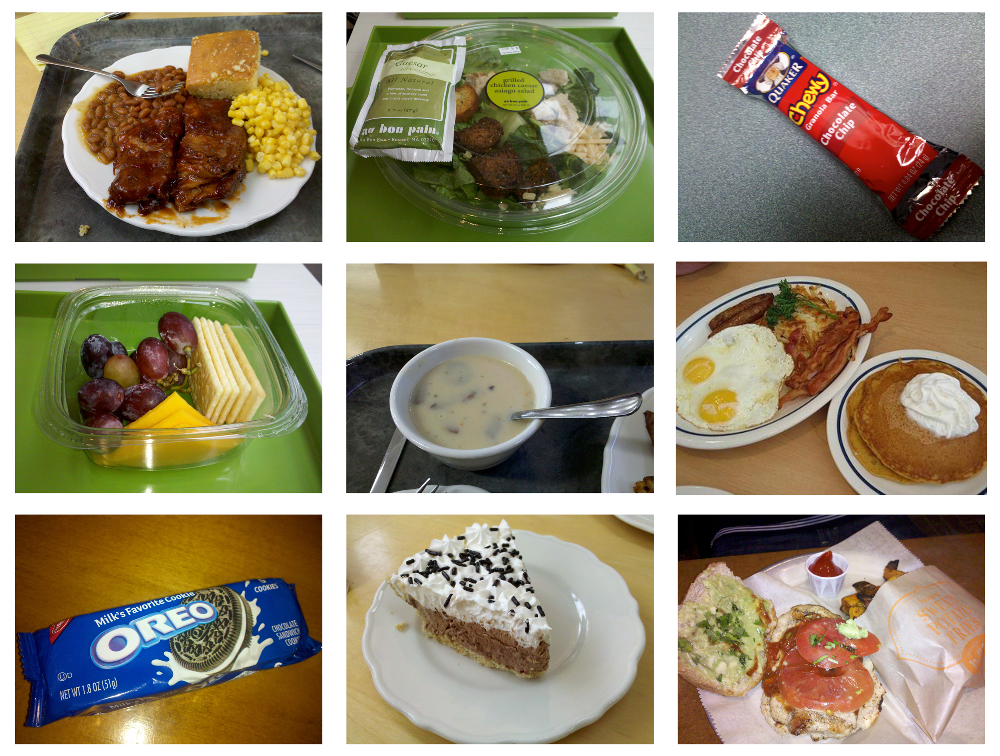
\includegraphics[width=\columnwidth]{figs/groundtruth.pdf}
   \caption{Examples of photos from the study of PlateMate's accuracy.}
   \label{fig:groundTruth}
\end{center}
\end{figure}

\subsubsection{Method}
We conducted the experiment with a sample of 18 photographs showing 36 distinct foods. Some depicted individual foods or packages, while others showed complex plates containing many items, as shown in Figure~\ref{fig:groundTruth}.  Each pictured food had nutritional data available through the manufacturer or preparer, and foods were weighed when necessary to ensure accuracy. These foods were selected to span a variety of meals and sources, including restaurants, cafeterias, and grocery items.  We also included a mix of simple foods and composite items like salads and sandwiches.

We recruited three professional dietitians to provide expert estimates: one was a private nutrition counselor, and the other two were employed by a hospital. They received compensation for their time and provided estimates from their own offices. They were encouraged to use any aids, like books and calorie databases, that they would typically use for a similar task.
% Note that their analysis is not directly comparable to the expert estimates in the original RFPM study~\cite{martin2009novel}. That experiment focused only on measuring portions, and experts were told what the foods were and provided with photographs of standard portions of each. Our study focused on genuine remote analysis, where experts had only the picture to work from. 

Our third set of estimates came from Meal Snap, a recent commercial application.  Meal Snap returns a range of calories rather than a definitive answer, so we used the mean of its high and low values.  

\begin{figure}
\begin{center}
   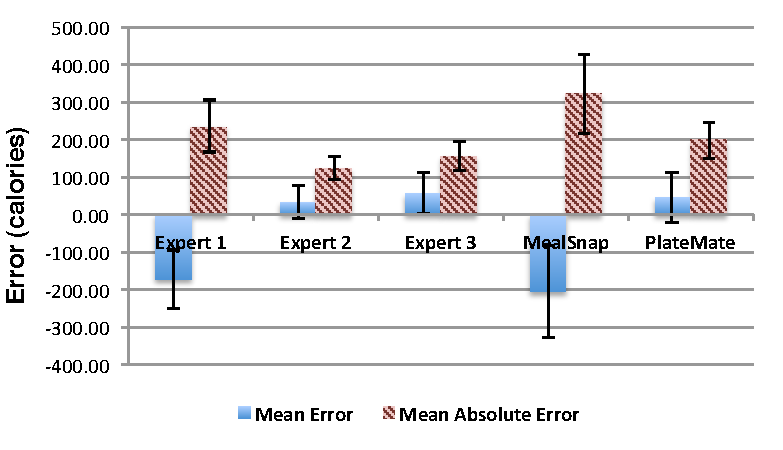
\includegraphics[width=\columnwidth]{figs/error-both}
   \caption{Mean errors (i.e., overall bias) and mean absolute errors (average magnitude of an error) for estimates made by the human experts, the Meal Snap application, and PlateMate compared to data provided by manufacturer or preparer.  Error bars correspond to standard error.}
   \label{fig:error}
\end{center}
\end{figure}

\subsubsection{Results}

In terms of mean absolute error on calorie estimates, PlateMate was not significantly different from the human experts or the Meal Snap application.  Figure~\ref{fig:error} illustrates the results in detail.  
As expected, trained dietitians were the most accurate on average. Their mean absolute error rates were $39.4\%$, $20.8\%$, and $26.1\%$, for an average of $172.0$ calories or $28.7\%$ per photograph. The best expert was off by just $124.5$ calories, on average. PlateMate was close behind with a mean absolute error rate of $198$ calories, or $33.2\%$.  MealSnap was farther behind, with an average error rate of $322.8$ calories or $53.9\%$.

Absolute error rates reflect the average magnitude of the error, but not the biases in each method. To understand how estimates from each source would add up over time, we also measured mean error without taking absolute values. The best expert overestimated by just 32.75 calories on average, for a mean error rate of $+5.5\%$.  The other two experts had error rates of $+9.2\%$ and $-27.5\%$.

%This result was in line with~\cite{martin2009novel}, which found trained nutritionists underestimated portions with an error rate of $-6.6\%$, though our task also required identifying the foods.

In comparison, PlateMate had a mean error rate of $+44.1$ calories, or $+7.4\%$, which was much closer than Meal Snap's $-34.4\%$. Expert and PlateMate results are significantly correlated with the ground truth data ($r^2 = .8626$, $.9062$, and $.9378$ for the experts, and $r^2=.8622$ for PlateMate, all with $p<.0001$), while Meal Snap results were not correlated with the actual nutritional content of the meals ($r^2=.2352$, $p=.3475$).
%MealSnap results appear almost completely uncorrelated with ground truth ($r^2=0.23$), while PlateMate and expert results were strongly correlated with actual calorie content of each food ($r^2=0.86$ and $0.93$, respectively). \bug[the $r^2$ for expert results, is this an average of the three experts?  Perhaps the better thing would be to show all three?]

%These results suggest that, while all three methods of remote food photography are somewhat inaccurate, PlateMate and experts are much better than MealSnap. MealSnap's results were almost random, while PlateMate and expert results tracked ground truth closely. PlateMate was less accurate than the best expert, but about the same as the mean.

PlateMate's error rate compares favorably to amateur self-reports, where error rates can be greater than $400$ calories/day and range from $-76\%$ to $+24\%$~\cite{schoeller1990inaccuracies,champagne2002energy}.  It also lacks the systematic bias towards underestimation in self-reports, especially among vulnerable users. These results indicate that PlateMate's answers, while imperfect, can be a useful nutritional guide.

\subsubsection{Error Analysis}

Most errors in the study corresponded to single failures in specific parts of the pipeline.   In the Tag stage, boxes were sometimes drawn improperly, leading to missing or duplicate identifications.  In one photo of a brownie and banana on a small plate, only one box was drawn covering the entire banana and most of the brownie.  As a result, the workers at the Identify stage omitted the brownie.  On a photo of a hamburger with mushrooms, overlapping boxes were drawn over the burger and topping.  In this case, the mushrooms were identified in both boxes.  

Most errors occurred in the Identify stage.  Turkers had trouble distinguishing similar types of a food, which sometimes had large nutrition differences.  A plate of vegetarian baked beans was identified as regular baked beans, tripling the calorie count.  Branded foods also caused problems: a relatively low-calorie chicken sandwich was identified as a sandwich from the restaurant Chili's, which had over twice as many calories.  Another common situation involved duplication with both a composite item and one or more foods included in that composite both being selected.  A slice of pizza with pepperoni and olives was identified as ``Pizza with Meat and Vegetables,'' ``Pepperoni,'' and ``Black Olives,'' duplicating the toppings.

During measurement, many very small quantities were overestimated, especially when a small amount of a food was spread over a large area.  A dash of parsley on a sandwich was overestimated as .27 cups, for example.  Other errors occurred when one food appeared in several boxes. This led to a hamburger bun being counted as two buns when each half of the bun was seen in its own box.

\subsection{User Study}
Our second study looked at the subjective experience of using PlateMate as an end-to-end system for nutritional monitoring, compared to manual logging.  We looked for insights about the system's usability, in terms of the inconvenience of taking photographs and the effort required to correct errors.  Finally, we wanted to observe how robustly PlateMate functioned in the ``real world,'' without any constraints on the types of photographs submitted to the system.

\subsubsection{Method}
We recruited 10 participants (4 male, 6 female) via advertisements posted on several university email lists.  Seven of the participants were undergraduates, two were graduate students, and one was a faculty member.

To help us evaluate the quality of the nutritional estimates generated by PlateMate and by the participants in this study, we recruited four dietitians employed at a local hospital.  Two of them had also participated in the experiment evaluating the accuracy of PlateMate, where they produced the most accurate results. Participants and dietitians were compensated for their time.

Users were interviewed before and after the experiment. In the first interview, we discussed prior experiences tracking meals and trained participants on using the system. In the exit interview, we discussed their experiences using both logging methods.  

During the study, we asked the participants to take photographs of their meals for four days and upload them to PlateMate once a day.  For two of the days, participants received estimates generated by PlateMate and could correct those estimates.  For the other two days, participants were not shown estimates and manually logged their food.  Half of the participants used the manual system first and half used PlateMate first.  We designed the interface for manual logging and correcting estimates to resemble existing commercial tools for manual food logging.

In order to assess the results produced by PlateMate compared to current consumer best practices, we used PlateMate to generate hidden estimates for participants' photos from the two days of manual recording.  Participants only saw this data during the exit interviews, when they were asked to compare their own logging with the automatic estimates.

\begin{figure}
\begin{center}
   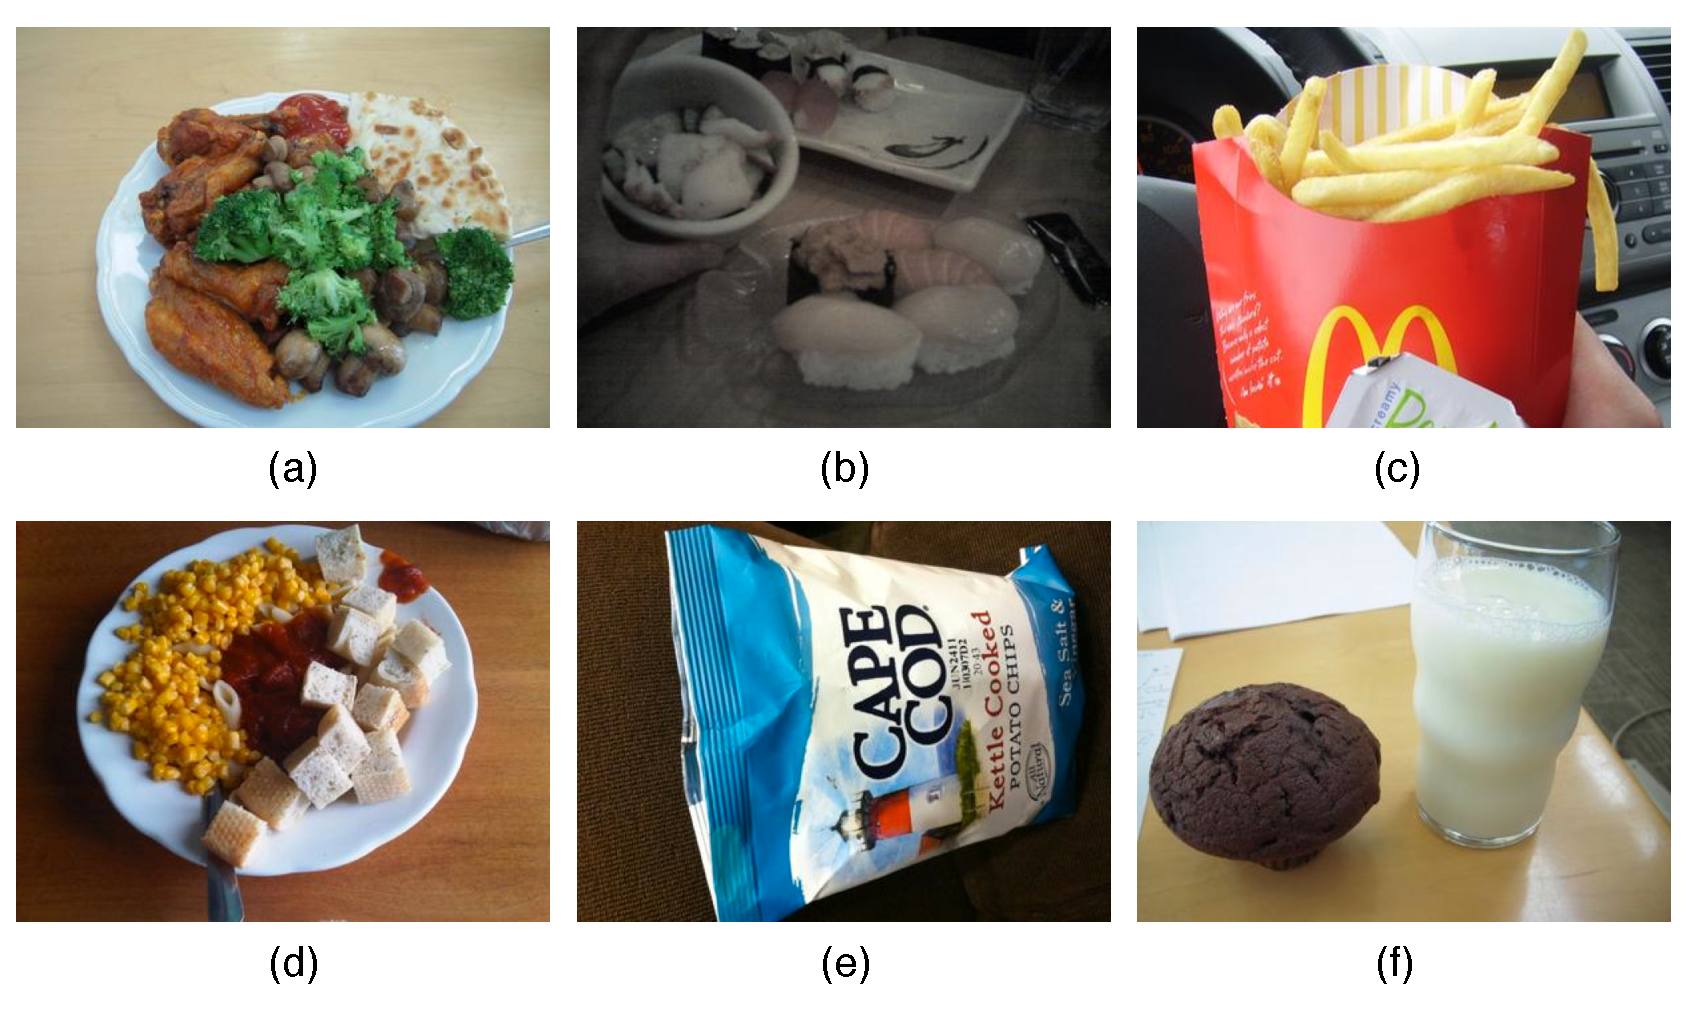
\includegraphics[width=\columnwidth]{figs/userphotos.pdf}
   \caption{Example user photos.  PlateMate handled (a) - (c) well, while (d) - (f) caused problems.  In (d) the pasta with sauce in the middle was hard to see; in (e) there is no sense of scale to determine the size of the bag; and in (f) the type of milk is unclear.}
   \label{fig:userPhotos}
\end{center}
\end{figure}

\subsubsection{Findings from the Initial Interviews}
Our pre-interviews with participants confirmed that existing methods of logging food are cumbersome. All but one of the 10 had tried logging their food at some point, but most gave up after a few days or weeks. Only two participants still tried, and neither reported doing so consistently or reliably. They recalled their attempts to keep track of food as ``annoying,'' ``inconvenient,'' and ``tedious.'' One subject recalled six separate failed attempts, each lasting just a few days. Some reported success when they were required to log for athletics or class projects, but recording lapsed when those commitments ended.

Despite these challenges, participants found nutritional information valuable. Eight participants reported looking at nutrition labels on packaged foods. Several reported looking up new foods out of curiosity. One participant reported revelations like ``Oh wow, that's a lot of calories in dressing,'' and another now dilutes her juice with water after discovering how much sugar it contains.

% I think this paragraph and the next can be cut. --EH
%Subjects acknowledged that finding this information is more difficult when foods are not packaged with labels. When eating prepared meals, especially in restaurants, they sometimes guessed crude nutrition estimates. Many had some background nutrition knowledge, which gave them a rough idea of the protein, fat, and carbohydrate levels of different kinds of foods. %One subject explained, ``When I'm at Subway getting a sandwich, I know if I get turkey and no cheese and a vinaigrette, it's better than getting the works because there's less fat.''

%Others relied on heuristics or rules of thumb for healthy eating, which don't require any systematic knowledge. Two subjects spoke of color variety and drawing from different food groups, emphasizing ``greens'' on the plate. Another spoke of eating ``like mom taught you.'' Others learned from their feelings after eating. One subject explained, ``I feel more grossed out at the fast food spots.''

\subsubsection{Exit Interview Reactions}
We asked all ten participants their preference between using PlateMate for automatic estimates and logging manually (by any method). Seven participants said they would prefer using PlateMate in the future, citing its ease of use and the convenience of ``having someone else do that for me rather than guess myself.'' One subject explained, ``My answers were closer to guesswork; this felt more like science.'' The three subjects who did not prefer PlateMate felt that they could not trust it or that the process of taking photos and correcting the estimates was too cumbersome.

Subjects were divided in their perceptions of PlateMate's
accuracy. Seven of 10 found the answers at least as good as their
own and of these four found PlateMate's estimates to be more accurate than self
reports.  After seeing his
own estimates and PlateMate's for the same meals, one subject said the
exercise ``confirmed my suspicions that you guys were more accurate
than I was. The tendency is always to say `oh, I didn't have that
much.''' Three others found their own estimates and PlateMate's
basically equivalent.

The other three subjects all found PlateMate less accurate than their
own estimates. One said that PlateMate's answers were close, ``like
$80$-$90\%$, but not perfect. I want to be sure.'' Another still
preferred PlateMate even though she could not fully trust its
results. She explained, ``For some people if it's not perfect they'll
never use it. But for me it was great...Even if it is only half of
them correct, that is fewer I have to enter manually, and the happier
I am.'' Another user disagreed, feeling that it took more effort to
correct PlateMate estimates than ``do it right myself the first
time.''

In total, seven users said that PlateMate required less effort than
manual logging, which most of these users considered unpleasant and
tedious. They called it ``annoying'', ``boring,'' and ``not
excruciating but not insignificant either.'' These participants said
PlateMate was ``definitely easier'' and ``much simpler,'' concluding
that it ``definitely saves me time and effort.'' They also found
receiving the results exciting. One user explained, ``it was more
fun...I got the email, and my friend was like, `Oh! Do we get to see
it now?''' Another was discouraged by the difficulty of manually
estimating portions, so she found it ``really helpful to have someone
else do that for me rather than guess myself.''

\subsubsection {PlateMate Performance}

Next, we analyze PlateMate's performance on photographs collected by
our users.  We wanted to investigate the system's robustness given a
broad variety of meals and realistic variations in photograph quality.
Ideally, the PlateMate estimates and manual logging data from the user
study could be compared to ground truth to determine accuracy, but
such data were clearly not available.

Instead, we first looked at the differences between participant and PlateMate estimates.  Comparing results from $112$ photos for which we had both participant and PlateMate estimates, we found the two sets of results to be positively correlated ($r^2=0.62$, $p<.0001$). PlateMate's estimates were slightly higher than participants', with a mean difference of $+41.0$ calories (median $+18.8$) or $+11.5\%$ that was not statistically significant (Wilcoxon $z=686$, {\it n.s.}). 

To gain further insight into relative accuracies of PlateMate and our participants, we presented 50 of these photographs together with both sets of nutritional estimates to 4 professional nutritionists.  The nutritionists worked in pairs.  Each pair was presented with a photo and two sets of numbers representing total calories, protein, fat, and carbohydrates.  One of these sets came from a participant and one from PlateMate, and the experts were blind to the source of the data.  They were then asked to pick the more accurate set, taking as much time as necessary and using any necessary tools and references.  The dietitians in each pair were allowed to talk to each other and could choose to agree on one data set as more accurate, disagree, or say they were unable to pick one data set as more accurate.  

%To verify the reliability of using human experts for this task, interspersed with the 50 photos from the user study were 10 photos from the ground truth study with one data set for the ground truth nutrition data and one an arbitrary error between 20\% and 50\% off of ground truth (the errors included both under- and overestimates).  Unfortunately, of the 10 ground truth photos, both pairs of dietitians picked the correct ground truth data set 50\% of the time, and we observed no bias toward either over- or underestimates.

Of the 50 user study photos, the first pair could not decide which set of nutritional estimates was more accurate in 5 cases and the second pair could not in 12 cases.  Out of the decisive photos, PlateMate data was selected as more accurate $44.4\%$ and $47.4\%$ of the time by the two pairs. These results suggest that neither method was obviously more accurate, especially since nearly half ($49.2\%$) of photos had estimates within 100 calories of each other.

% Do we need this paragraph? We're undecided. - JN
When disagreements did happen, PlateMate's estimates were larger $63.5\%$ of the time. This is consistent with our finding in the first study that PlateMate slightly overestimates and prior research that suggests a strong bias in manual recording towards underestimation.~\cite{pikholz2004under,goris2000undereating}.  PlateMate's estimates for daily energy intake were $+229.8$ calories higher than self-reports on average, a difference equivalent to four Oreo cookies every day.

\subsubsection{Error Analysis}
Many of the errors seen from the user study results were similar to those already discussed from the ground truth study, but some new issues emerged.  In measurement, we saw difficulty estimating portions when extreme close-up photos were taken with no sense of scale.  Turkers could not agree if a bag of potato chips (Figure~\ref{fig:userPhotos}) was a portion or large bag.  Scale was also a problem in identification: a small tangerine was identified as a larger orange.  Other identification errors occurred when foods with nearly correct names but vastly different nutrition were selected, like ``grapefruit juice'' and ``juice concentrate,'' which has eight times the calories. One Subway chicken sandwich was identified as ``Subway Roasted Chicken Patty,'' which could be interpreted as the whole sandwich but in fact just contained the chicken.

Human errors during manual logging mostly occurred when participants forgot to log a certain food.  In photo (f) of Figure~\ref{fig:userPhotos} the participant only recorded the milk and forgot to log the muffin, which represented most of the photo's calories.  In a photo of french fries, a participant forgot to record the dipping sauce next to the fries.  Similar errors occurred when participants sought to simplify their recordings to save time.  One subject ate a bowl of several types of fruit but recorded the entire bowl as raspberries, while PlateMate correctly identified each fruit.

\subsubsection{Cost and Wait Times}
During the course of both evaluations we analyzed 262 photos using PlateMate, generating 1,553 HITs that were assigned to 199 total Turkers 4,332 times.  The average cost of a single photo was \$1.40.  The mean time to complete analysis was 94.14 minutes, with 73\% of photos completing in less than 2 hours and all photos completing in less than 6 hours.

\section{DISCUSSION AND FUTURE DIRECTIONS}

%This section considers several successes and failures of PlateMate and opportunities for related work in crowdsourced remote food photography and crowdsourcing at large.  
The results from our evaluations of PlateMate suggest that through careful coordination, untrained workers can approach experts in their accuracy in estimating nutrition information from photographs of meals. These estimates are close to those logged by the people who actually ate the meals. However, several issues which became apparent during the course of our evaluations could be addressed through future work.

PlateMate consistently struggled to produce good results on liquids like beverages and salad dressing. One participant drinks a low-fat latte each morning, but PlateMate consistently identified it as coffee with cream.  Another only used low-fat salad dressings, which were identified as their full-fat versions.  These issues could be addressed by introducing personalization mechanisms.  For example, the interface could give users access to images of foods they eat frequently---instead of taking a picture of today's latte, a user would simply select a picture of last week's, ensuring correct logging and obviating the need for engaging the crowd. Statistical methods could also be used to adapt the Turker interface to emphasize the foods most common in a user's diet and thus most likely to appear in their photos.  These approaches could result in improvements to both reliability and cost.

%Two approaches in future work could address this type of issue.  First, allowing users to denote ``favorite foods'' could both provide guides for Turkers during the Identify stage and make it faster for users to select these items when correcting estimates.  A more involved approach could also utilize machine learning based on users' corrections to either guide workers to select the items more likely to be chosen by each user or automatically correct estimates which appear to replicate past mistakes.

%Unsurprisingly, nearly all subjects were frustrated by the effort required to transfer photos to a computer and manually upload them to PlateMate. Many commented that a smartphone application to combine photography, uploading, and receiving estimates would simplify this process.  In addition to a smartphone application replicating our online interface, interesting future work exists around location.  

Geolocation capabilities available in many mobile devices could be used to further improve accuracy of the crowdsourced analysis of restaurant meals. Photos could be annotated with the cuisine of the restaurant in which they were taken, providing Turkers with helpful context while maintaining the privacy of user's actual location.  Integrating with existing local ``check-in'' applications like Foursquare\footnote{\url{https://foursquare.com/}} would make it even simpler to associate meals with their places of origin.
% could also provide a means to retrieve meals later if one forgot to take a picture or felt that taking a picture would be socially awkward---would require that a person marks a location without taking a pic

\newcontent{Permitting optional textual annotations by users (e.g., ``skim latte'', ``mango curry'') would naturally further improve accuracy and reduce cost.  So would employing computer vision and machine learning for parts of the process:}  over time and continued use, PlateMate could build a large database mapping tagged sections of photographs to specific foods and portions.  An algorithmic approach could be taken to analyze new photos for similarity with previously processed images.  This could result in fully computerized analysis based on the prior crowdsourced work, extending the vision approach in~\cite{kitamura2010image}, or these potential similar items could be surfaced in alternate HIT interfaces to Turkers as a way of skipping unnecessary stages of the PlateMate process.

\newcontent{This work was done on the assumption that lowering the barrier to monitoring one's food intake may result in a larger number of people persisting in their attempts to alter their eating habits.  We are aware, however, that making the process too easy may reduce the opportunities for reflection.  Ultimately, PlateMate's success depends on the users' willingness to engage with the information it provides.  But if they do, PlateMate can help its users correct misconceptions about nutritional content of the foods they consume and to improve their ability to estimate portion sizes.}

The Remote Food Photography Method relies on two images of each meal:
a photograph of the original portion and a photograph of any food that was left
uneaten. We have explored the first part of the process and we expect
that the second can be performed in a similar manner.  A major difficulty in analyzing images of
leftovers is likely to be in identifying the foods in the photo. But
as such foods are already identified in the first part of the process, a reasonable approach to extend PlateMate may be to display an annotated
image of the original plate next to the photograph of the
leftovers, and ask Turkers to identify portions of the second image where the
original foods are present and, in the subsequent step, to estimate the
amounts of the leftover foods. Our future work will aim to test the efficacy
of such an approach and to thus fully implement the Remote Food Photography Method.
%By combining algorithmic and crowdsourcing approaches, these types of extensions could allow PlateMate to reach higher accuracy.  They also suggest a different type of role for human computation than what has been suggested in prior work.  While this paper has focused solely on crowdsourcing nutrition analysis, future evolutions of this system could use Mechanical Turk as one part of a larger hole, in which human workers build training datasets for learning algorithms and are automatically employed to cover other gaps in automated algorithms.

%\fix{hq: I am also ok with cut below}
%\cut{Finally, our work focused on providing an accurate and unobtrusive way of measuring a user's eating habits. Other work has explored how accurate sensing of a user's behavior can be used to motivate positive behavior change.  UbiFit, Houston, and Fish'n'Steps use personal displays, games, and social networks to encourage physical activity~\cite{Consolvo:2008:FRA:1409635.1409644,Consolvo:2006:DRT:1124772.1124840,Lin:2006fk}, while projects like UbiGreen apply similar principles to promoting sustainable activities~\cite{Froehlich:2009:UIM:1518701.1518861}.  PlateMate can enable these techniques to be used to help people make healthier eating choices.
%}

\section{CONCLUSION}

This paper presents PlateMate, which allows users to take photos of their meals and receive estimates of the meals' nutrition content.  PlateMate builds on a concept of remote food photography developed recently by the nutrition community.  While the original method relies on expert dietitians providing the estimates, PlateMate uses Amazon Mechanical Turk to make this approach more affordable and scalable.  

Through careful decomposition of the process into small and verifiable steps, PlateMate achieves accuracy comparable to trained dietitians:  
the results of our evaluation demonstrate that PlateMate overestimated caloric content by $+7.4\%$ on average, while the best of three trained dietitians overestimated by $+5.5\%$.  In our user study, which compared PlateMate to the currently most common practice of manual self-logging of meals, most participants found PlateMate easier and faster to use and at least as accurate.  Four dietitians were unable to differentiate between nutrition estimates produced by PlateMate and those manually logged by our study participants, further suggesting parity with the current methods.

Overall, PlateMate is an attractive alternative to existing solutions because it reduces user effort compared to manual logging, achieves good accuracy, is affordable, and can be conceivably deployed to support a large number of users.

We suggest ways in which the accuracy can be further improved and cost reduced by combining crowdsourcing with machine learning, computer vision, personalization and location information. 

PlateMate is one of the first complex crowdsourcing systems to combine---in a real world application---several of the recently introduced design patterns for programming the crowds.  In the process of building PlateMate, we have developed the Management framework, a modular software framework inspired by the structure of human organizations.  The Manager abstraction conveniently supported hierarchical problem decomposition as well as modular development and debugging.  The choice of message passing as the main communication mechanism cleanly supports asynchronous just-in-time processing of sub-tasks.  PlateMate may serve as a useful case study for future developers of complex crowd-based applications.

%The patterns and techniques used by PlateMate to approach expert-level accuracy with untrained workers could enable further work in both persuasive technologies and other crowdsourcing challenges.



% bibliography --- please add new references to the platemate.bib
%\small % a little space saving device
\begin{flushleft}
\bibliographystyle{unm}
\bibliography{platemate,kzg}
\end{flushleft}

\end{document}

\section{THE MANAGEMENT FRAMEWORK}
In this section, we introduce a programming framework for solving
problems with crowds based on a human organizational hierarchy. This
approach differs conceptually from prior work, which has focused on
creating ``crowd programming languages'' that combine human and
machine computation. For example, TurKit~\cite{little2010turkit} lets requesters
program crowds in JavaScript, Qurk~\cite{qurk} integrated crowds into
SQL, and CrowdForge~\cite{crowdforge} parallelized work with MapReduce
scripts. In each case, these toolkits have attempted to make working
with crowds more like working with computers.
This approach emphasizes computation as the natural glue for combining individual worker contributions and the resulting artifact is a computer program with some of the primitive operations implemented as ``functional calls'' to human workers~\cite{little2010turkit}.

Because PlateMate relies primarily on human work, divided into a number of heterogenous and interacting tasks, and because the issues of worker skill and motivation were central to our design process, we found it conceptually helpful to use human organizational hierarchies as the metaphor for designing our system.  Specifically, we observe that in the real world, expert-level work (e.g., building a table) can be reproduced by less skilled workers---each working on a specific part of the process---supervised by managers who are not necessarily skilled craftsmen themselves, but who know how to assign tasks, route work among workers, and verify the quality of the work.

%To illustrate, in the real world, expert-level work can be reproduced by less skilled workers
%through division of labor in an organized hierarchy. Large, complex
%goals are decomposed into simpler operations overseen by managers who
%supervise workers with clear areas of responsibility. Consider making
%a table. One approach is to have a highly-trained expert craftsman
%build the table alone. Alternatively, a factory can build a table by
%assigning each worker a small piece of the job. One worker may saw
%the wood, another may polish it, and a third may assemble the
%pieces together. Supervisors---who need not be experts, either---assign tasks to workers, route work between them, and verify the quality of work. 

%Such approach is conceptually useful for processing large computational tasks with human
%intelligence as an extra ``functional call''~\cite{little2010turkit}. 

%PlateMate,
%however, aims to emulate the reasoning of an individual human
%expert. In this domain, we found the abstraction of ``programming
%crowds'' as if they were computers unnatural. 
%We could not think of
%the crowd as a function call, since our HITs and workflows were based
%on careful observation of Turker psychology and motivation. 
%Instead, 
%PlateMate
%thus follows the opposite approach. 

%With PlateMate, however, we 
%
%PlateMate tries to make programming crowds more like instructing and
%organizing a team of humans.


%This approach of distributing
%work has been profoundly successful with material goods, and we seek
%to do the same thing with expert thought and reasoning.\fix{Consider removing this last sentence -- this is a broad claim with no citations.}



%\section{The Management Framework}
Thus, to implement division of labor for crowdsourcing, we created a new
framework organized around objects called \em managers.\em\  
%Managers are independent of their peers.  
%written as if they are independent agents in a distributed system. 
Managers communicate with their supervisors and their \em employees \em using asynchronous message passing: managers assign tasks by placing them in inboxes of lower level managers and communicate with their superiors by placing results of completed tasks in their own outboxes.
%They constantly check for new assignments, assign work to
%their \em employees,\em\ receive completed work, and send their own outputs up
%the hierarchy. 
This hierarchical message-passing approach allows programmers
to implement workflows by decomposing problems into progressively
smaller steps.

As illustrated earlier in Figure~\ref{fig:system}, the root of this tree is a \em chief \em manager, which gathers new inputs
and produces completed outputs. In PlateMate, the chief has three
employees: Tag, Identify, and Measure. Each of these are in turn
managers and have their own employees, corresponding to the individual
HITs described above.

This hierarchical structure creates a flexible workflow consisting of
 modules connected by higher-level managers. Managers can route work intelligently among their
employees, and may dynamically alter the sequence of steps in the process depending on a situation. For example, PlateMate's Tag manager compares the outputs from its
DrawBoxes employee. If they are sufficiently different, they are sent
to the VoteBoxes manager to decide between them. Otherwise, one answer
is chosen randomly and sent up the hierarchy as Tag's completed
output. All managers work in parallel, each processing its own stream of
work. 

When multiple tasks are submitted, processing is done just-in-time: for example, as soon as one photograph is tagged, the Identify manager begins the process of finding out what foods are present in each of the boxes without waiting for the remaining photographs to be tagged.  

%This asynchronous approach improves on the iterative workflows
%in TurKit, where each stage blocks until every task in that stage has
%been completed. 
%It also differs from CrowdForge, where intermediate
%outputs must all be finished before they can be recombined. Instead,
%completed work is sent up the chain and on to the next step
%immediately, where another manager can begin to process it.

At the lowest level of the hierarchy are managers whose employees are
the crowd workers. Managers at this level create jobs (such as asking
for the food in one tagged box on a photo to be identified) and
receive responses. Programmers create HIT templates and validation
functions which are used by the framework to create HITs and approve
work. Managers simply assign work to the crowd and receive validated outputs that can be passed up the
tree.

Of course, the Management Framework \em is \em a computational framework, and it naturally supports a number of the recently introduced design patterns for programming the crowds.  For example, the Tag step is an analog of the map step in MapReduce and the Describe step (part of Identify, see Figure~\ref{fig:system}) relies on iterative refinement~\cite{little10:exploring} to improve the level of detail of the descriptions.

Management is implemented as an extension of Django, a web application
framework for Python. It builds on several useful features from
Django, including an HTML template language for defining HIT
instructions, examples, and interfaces. It also uses Django's
object-relational mapper, which automatically stores Python objects in
a MySQL database. This means that the precise state of the system is
always stored, including managers' inboxes and outboxes, active HITs
and completed assignments, and intermediate inputs and outputs. This
simplifies later analysis, since requesters can go back and query
responses from each stage in the workflow. It also protects completed
work from program errors or service outages; after crashes, execution simply  
resumes from the last good state. 
%\fix{drop this: ``rather than restarting from the
%beginning as in TurKit's crash-and-rerun
%model~\cite{little2010turkit}.'' -- turkit doesn't really start from the beginning, it also picks up where 
%you leave off}



\section{EVALUATION}

Our evaluation focused on PlateMate's feasibility as a replacement for traditional food logging.  We considered three broad criteria:
\vspace*{-2mm}
\begin{enumerate}
\item \textbf{Accuracy.} How accurate were crowdsourced estimates compared to current alternatives? Could users trust them?
\item \textbf{Usability.} How much effort or discomfort would users experience in photographing food, uploading the photos, and correcting errors in PlateMate's estimates?
\item \textbf{Robustness.} How well does the PlateMate system fare with ``real world'' photographs?
\end{enumerate}
\vspace*{-2mm}
We designed two experiments to answer these questions.  In the first, nutrition data returned from PlateMate was compared with ground truth, expert dietitian estimates, and a recent commercial application.  In the second study, ten participants used PlateMate and a manual food-logging system for four days.

\subsection{Evaluation of Accuracy}

Our first study had two goals. The first was to determine the accuracy of PlateMate with ground truth data obtained from manufacturers or preparers. The second was to compare PlateMate's performance with two alternative approaches to remote food photography: analysis by experts and results from Meal Snap.  
\newcontent{Because Meal Snap only returns calorie information and to make the task manageable for our expert participants, we limited our comparison to estimated calories even though PlateMate generates reports that also include fat, protein, and carbohydrates.}

\begin{figure}
\begin{center}
   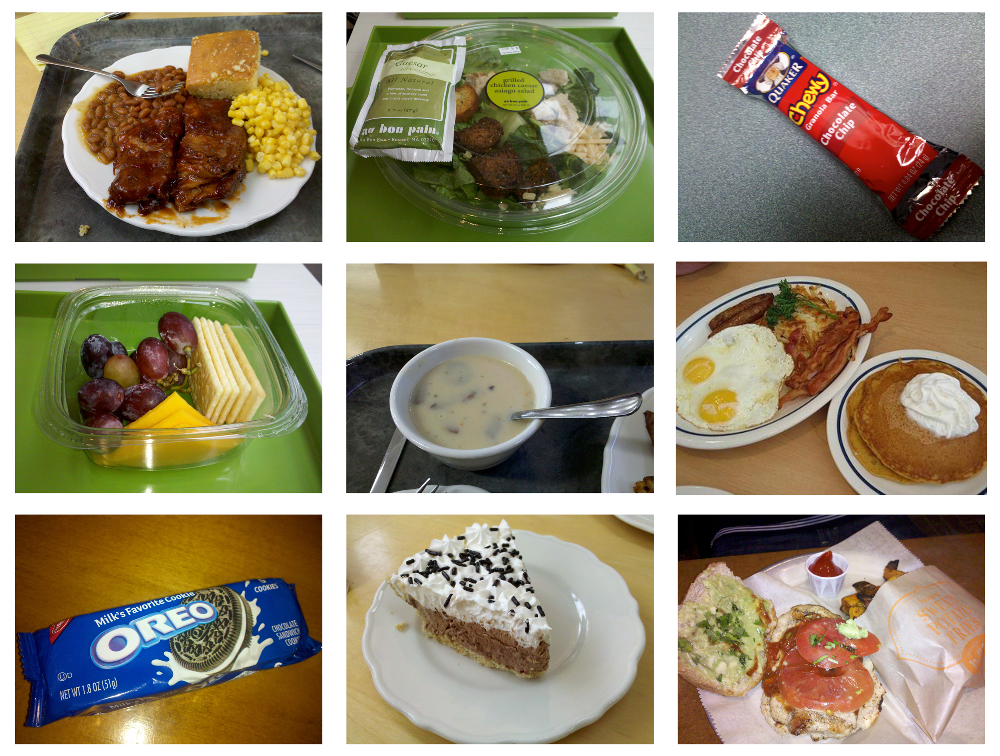
\includegraphics[width=\columnwidth]{figs/groundtruth.pdf}
   \caption{Examples of photos from the study of PlateMate's accuracy.}
   \label{fig:groundTruth}
\end{center}
\end{figure}

\subsubsection{Method}
We conducted the experiment with a sample of 18 photographs showing 36 distinct foods. Some depicted individual foods or packages, while others showed complex plates containing many items, as shown in Figure~\ref{fig:groundTruth}.  Each pictured food had nutritional data available through the manufacturer or preparer, and foods were weighed when necessary to ensure accuracy. These foods were selected to span a variety of meals and sources, including restaurants, cafeterias, and grocery items.  We also included a mix of simple foods and composite items like salads and sandwiches.

We recruited three professional dietitians to provide expert estimates: one was a private nutrition counselor, and the other two were employed by a hospital. They received compensation for their time and provided estimates from their own offices. They were encouraged to use any aids, like books and calorie databases, that they would typically use for a similar task.
% Note that their analysis is not directly comparable to the expert estimates in the original RFPM study~\cite{martin2009novel}. That experiment focused only on measuring portions, and experts were told what the foods were and provided with photographs of standard portions of each. Our study focused on genuine remote analysis, where experts had only the picture to work from. 

Our third set of estimates came from Meal Snap, a recent commercial application.  Meal Snap returns a range of calories rather than a definitive answer, so we used the mean of its high and low values.  

\begin{figure}
\begin{center}
   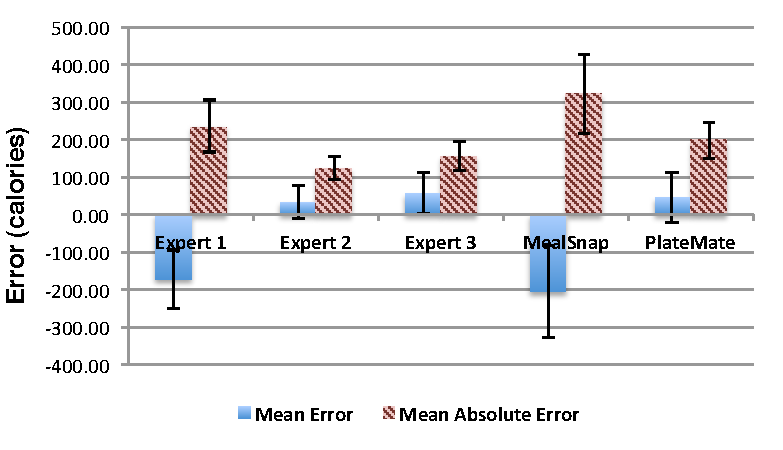
\includegraphics[width=\columnwidth]{figs/error-both}
   \caption{Mean errors (i.e., overall bias) and mean absolute errors (average magnitude of an error) for estimates made by the human experts, the Meal Snap application, and PlateMate compared to data provided by manufacturer or preparer.  Error bars correspond to standard error.}
   \label{fig:error}
\end{center}
\end{figure}

\subsubsection{Results}

In terms of mean absolute error on calorie estimates, PlateMate was not significantly different from the human experts or the Meal Snap application.  Figure~\ref{fig:error} illustrates the results in detail.  
As expected, trained dietitians were the most accurate on average. Their mean absolute error rates were $39.4\%$, $20.8\%$, and $26.1\%$, for an average of $172.0$ calories or $28.7\%$ per photograph. The best expert was off by just $124.5$ calories, on average. PlateMate was close behind with a mean absolute error rate of $198$ calories, or $33.2\%$.  MealSnap was farther behind, with an average error rate of $322.8$ calories or $53.9\%$.

Absolute error rates reflect the average magnitude of the error, but not the biases in each method. To understand how estimates from each source would add up over time, we also measured mean error without taking absolute values. The best expert overestimated by just 32.75 calories on average, for a mean error rate of $+5.5\%$.  The other two experts had error rates of $+9.2\%$ and $-27.5\%$.

%This result was in line with~\cite{martin2009novel}, which found trained nutritionists underestimated portions with an error rate of $-6.6\%$, though our task also required identifying the foods.

In comparison, PlateMate had a mean error rate of $+44.1$ calories, or $+7.4\%$, which was much closer than Meal Snap's $-34.4\%$. Expert and PlateMate results are significantly correlated with the ground truth data ($r^2 = .8626$, $.9062$, and $.9378$ for the experts, and $r^2=.8622$ for PlateMate, all with $p<.0001$), while Meal Snap results were not correlated with the actual nutritional content of the meals ($r^2=.2352$, $p=.3475$).
%MealSnap results appear almost completely uncorrelated with ground truth ($r^2=0.23$), while PlateMate and expert results were strongly correlated with actual calorie content of each food ($r^2=0.86$ and $0.93$, respectively). \bug[the $r^2$ for expert results, is this an average of the three experts?  Perhaps the better thing would be to show all three?]

%These results suggest that, while all three methods of remote food photography are somewhat inaccurate, PlateMate and experts are much better than MealSnap. MealSnap's results were almost random, while PlateMate and expert results tracked ground truth closely. PlateMate was less accurate than the best expert, but about the same as the mean.

PlateMate's error rate compares favorably to amateur self-reports, where error rates can be greater than $400$ calories/day and range from $-76\%$ to $+24\%$~\cite{schoeller1990inaccuracies,champagne2002energy}.  It also lacks the systematic bias towards underestimation in self-reports, especially among vulnerable users. These results indicate that PlateMate's answers, while imperfect, can be a useful nutritional guide.

\subsubsection{Error Analysis}

Most errors in the study corresponded to single failures in specific parts of the pipeline.   In the Tag stage, boxes were sometimes drawn improperly, leading to missing or duplicate identifications.  In one photo of a brownie and banana on a small plate, only one box was drawn covering the entire banana and most of the brownie.  As a result, the workers at the Identify stage omitted the brownie.  On a photo of a hamburger with mushrooms, overlapping boxes were drawn over the burger and topping.  In this case, the mushrooms were identified in both boxes.  

Most errors occurred in the Identify stage.  Turkers had trouble distinguishing similar types of a food, which sometimes had large nutrition differences.  A plate of vegetarian baked beans was identified as regular baked beans, tripling the calorie count.  Branded foods also caused problems: a relatively low-calorie chicken sandwich was identified as a sandwich from the restaurant Chili's, which had over twice as many calories.  Another common situation involved duplication with both a composite item and one or more foods included in that composite both being selected.  A slice of pizza with pepperoni and olives was identified as ``Pizza with Meat and Vegetables,'' ``Pepperoni,'' and ``Black Olives,'' duplicating the toppings.

During measurement, many very small quantities were overestimated, especially when a small amount of a food was spread over a large area.  A dash of parsley on a sandwich was overestimated as .27 cups, for example.  Other errors occurred when one food appeared in several boxes. This led to a hamburger bun being counted as two buns when each half of the bun was seen in its own box.

\subsection{User Study}
Our second study looked at the subjective experience of using PlateMate as an end-to-end system for nutritional monitoring, compared to manual logging.  We looked for insights about the system's usability, in terms of the inconvenience of taking photographs and the effort required to correct errors.  Finally, we wanted to observe how robustly PlateMate functioned in the ``real world,'' without any constraints on the types of photographs submitted to the system.

\subsubsection{Method}
We recruited 10 participants (4 male, 6 female) via advertisements posted on several university email lists.  Seven of the participants were undergraduates, two were graduate students, and one was a faculty member.

To help us evaluate the quality of the nutritional estimates generated by PlateMate and by the participants in this study, we recruited four dietitians employed at a local hospital.  Two of them had also participated in the experiment evaluating the accuracy of PlateMate, where they produced the most accurate results. Participants and dietitians were compensated for their time.

Users were interviewed before and after the experiment. In the first interview, we discussed prior experiences tracking meals and trained participants on using the system. In the exit interview, we discussed their experiences using both logging methods.  

During the study, we asked the participants to take photographs of their meals for four days and upload them to PlateMate once a day.  For two of the days, participants received estimates generated by PlateMate and could correct those estimates.  For the other two days, participants were not shown estimates and manually logged their food.  Half of the participants used the manual system first and half used PlateMate first.  We designed the interface for manual logging and correcting estimates to resemble existing commercial tools for manual food logging.

In order to assess the results produced by PlateMate compared to current consumer best practices, we used PlateMate to generate hidden estimates for participants' photos from the two days of manual recording.  Participants only saw this data during the exit interviews, when they were asked to compare their own logging with the automatic estimates.

\begin{figure}
\begin{center}
   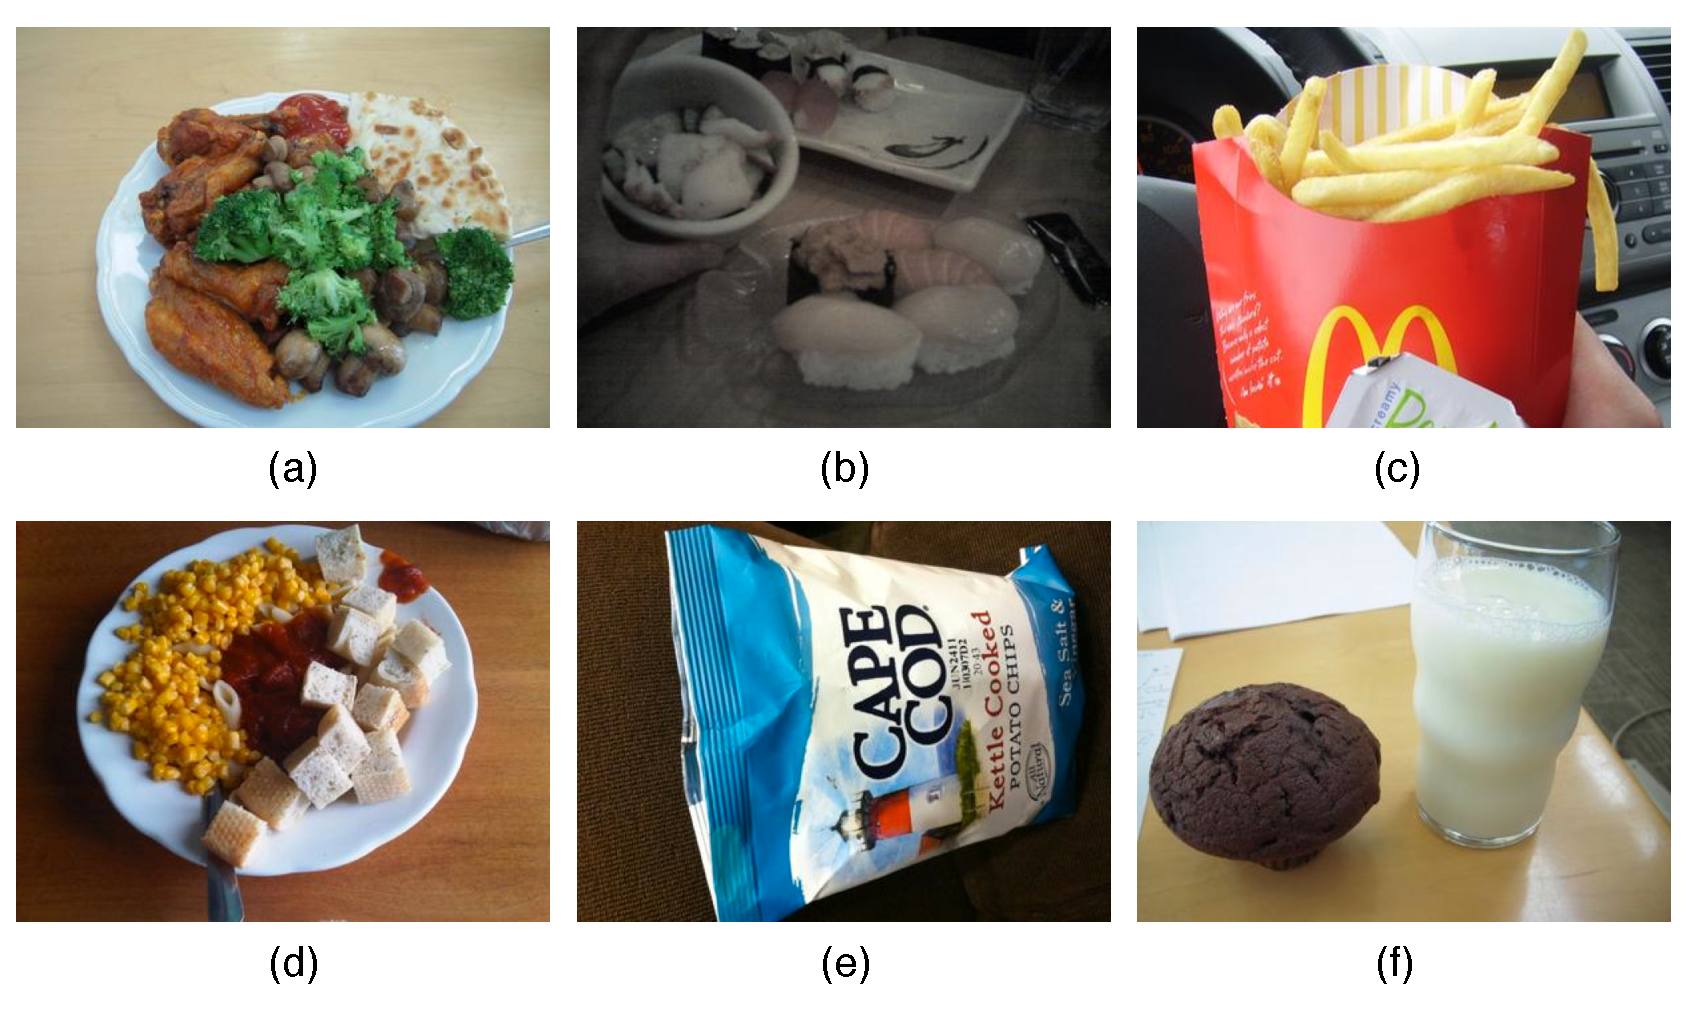
\includegraphics[width=\columnwidth]{figs/userphotos.pdf}
   \caption{Example user photos.  PlateMate handled (a) - (c) well, while (d) - (f) caused problems.  In (d) the pasta with sauce in the middle was hard to see; in (e) there is no sense of scale to determine the size of the bag; and in (f) the type of milk is unclear.}
   \label{fig:userPhotos}
\end{center}
\end{figure}

\subsubsection{Findings from the Initial Interviews}
Our pre-interviews with participants confirmed that existing methods of logging food are cumbersome. All but one of the 10 had tried logging their food at some point, but most gave up after a few days or weeks. Only two participants still tried, and neither reported doing so consistently or reliably. They recalled their attempts to keep track of food as ``annoying,'' ``inconvenient,'' and ``tedious.'' One subject recalled six separate failed attempts, each lasting just a few days. Some reported success when they were required to log for athletics or class projects, but recording lapsed when those commitments ended.

Despite these challenges, participants found nutritional information valuable. Eight participants reported looking at nutrition labels on packaged foods. Several reported looking up new foods out of curiosity. One participant reported revelations like ``Oh wow, that's a lot of calories in dressing,'' and another now dilutes her juice with water after discovering how much sugar it contains.

% I think this paragraph and the next can be cut. --EH
%Subjects acknowledged that finding this information is more difficult when foods are not packaged with labels. When eating prepared meals, especially in restaurants, they sometimes guessed crude nutrition estimates. Many had some background nutrition knowledge, which gave them a rough idea of the protein, fat, and carbohydrate levels of different kinds of foods. %One subject explained, ``When I'm at Subway getting a sandwich, I know if I get turkey and no cheese and a vinaigrette, it's better than getting the works because there's less fat.''

%Others relied on heuristics or rules of thumb for healthy eating, which don't require any systematic knowledge. Two subjects spoke of color variety and drawing from different food groups, emphasizing ``greens'' on the plate. Another spoke of eating ``like mom taught you.'' Others learned from their feelings after eating. One subject explained, ``I feel more grossed out at the fast food spots.''

\subsubsection{Exit Interview Reactions}
We asked all ten participants their preference between using PlateMate for automatic estimates and logging manually (by any method). Seven participants said they would prefer using PlateMate in the future, citing its ease of use and the convenience of ``having someone else do that for me rather than guess myself.'' One subject explained, ``My answers were closer to guesswork; this felt more like science.'' The three subjects who did not prefer PlateMate felt that they could not trust it or that the process of taking photos and correcting the estimates was too cumbersome.

Subjects were divided in their perceptions of PlateMate's
accuracy. Seven of 10 found the answers at least as good as their
own and of these four found PlateMate's estimates to be more accurate than self
reports.  After seeing his
own estimates and PlateMate's for the same meals, one subject said the
exercise ``confirmed my suspicions that you guys were more accurate
than I was. The tendency is always to say `oh, I didn't have that
much.''' Three others found their own estimates and PlateMate's
basically equivalent.

The other three subjects all found PlateMate less accurate than their
own estimates. One said that PlateMate's answers were close, ``like
$80$-$90\%$, but not perfect. I want to be sure.'' Another still
preferred PlateMate even though she could not fully trust its
results. She explained, ``For some people if it's not perfect they'll
never use it. But for me it was great...Even if it is only half of
them correct, that is fewer I have to enter manually, and the happier
I am.'' Another user disagreed, feeling that it took more effort to
correct PlateMate estimates than ``do it right myself the first
time.''

In total, seven users said that PlateMate required less effort than
manual logging, which most of these users considered unpleasant and
tedious. They called it ``annoying'', ``boring,'' and ``not
excruciating but not insignificant either.'' These participants said
PlateMate was ``definitely easier'' and ``much simpler,'' concluding
that it ``definitely saves me time and effort.'' They also found
receiving the results exciting. One user explained, ``it was more
fun...I got the email, and my friend was like, `Oh! Do we get to see
it now?''' Another was discouraged by the difficulty of manually
estimating portions, so she found it ``really helpful to have someone
else do that for me rather than guess myself.''

\subsubsection {PlateMate Performance}

Next, we analyze PlateMate's performance on photographs collected by
our users.  We wanted to investigate the system's robustness given a
broad variety of meals and realistic variations in photograph quality.
Ideally, the PlateMate estimates and manual logging data from the user
study could be compared to ground truth to determine accuracy, but
such data were clearly not available.

Instead, we first looked at the differences between participant and PlateMate estimates.  Comparing results from $112$ photos for which we had both participant and PlateMate estimates, we found the two sets of results to be positively correlated ($r^2=0.62$, $p<.0001$). PlateMate's estimates were slightly higher than participants', with a mean difference of $+41.0$ calories (median $+18.8$) or $+11.5\%$ that was not statistically significant (Wilcoxon $z=686$, {\it n.s.}). 

To gain further insight into relative accuracies of PlateMate and our participants, we presented 50 of these photographs together with both sets of nutritional estimates to 4 professional nutritionists.  The nutritionists worked in pairs.  Each pair was presented with a photo and two sets of numbers representing total calories, protein, fat, and carbohydrates.  One of these sets came from a participant and one from PlateMate, and the experts were blind to the source of the data.  They were then asked to pick the more accurate set, taking as much time as necessary and using any necessary tools and references.  The dietitians in each pair were allowed to talk to each other and could choose to agree on one data set as more accurate, disagree, or say they were unable to pick one data set as more accurate.  

%To verify the reliability of using human experts for this task, interspersed with the 50 photos from the user study were 10 photos from the ground truth study with one data set for the ground truth nutrition data and one an arbitrary error between 20\% and 50\% off of ground truth (the errors included both under- and overestimates).  Unfortunately, of the 10 ground truth photos, both pairs of dietitians picked the correct ground truth data set 50\% of the time, and we observed no bias toward either over- or underestimates.

Of the 50 user study photos, the first pair could not decide which set of nutritional estimates was more accurate in 5 cases and the second pair could not in 12 cases.  Out of the decisive photos, PlateMate data was selected as more accurate $44.4\%$ and $47.4\%$ of the time by the two pairs. These results suggest that neither method was obviously more accurate, especially since nearly half ($49.2\%$) of photos had estimates within 100 calories of each other.

% Do we need this paragraph? We're undecided. - JN
When disagreements did happen, PlateMate's estimates were larger $63.5\%$ of the time. This is consistent with our finding in the first study that PlateMate slightly overestimates and prior research that suggests a strong bias in manual recording towards underestimation.~\cite{pikholz2004under,goris2000undereating}.  PlateMate's estimates for daily energy intake were $+229.8$ calories higher than self-reports on average, a difference equivalent to four Oreo cookies every day.

\subsubsection{Error Analysis}
Many of the errors seen from the user study results were similar to those already discussed from the ground truth study, but some new issues emerged.  In measurement, we saw difficulty estimating portions when extreme close-up photos were taken with no sense of scale.  Turkers could not agree if a bag of potato chips (Figure~\ref{fig:userPhotos}) was a portion or large bag.  Scale was also a problem in identification: a small tangerine was identified as a larger orange.  Other identification errors occurred when foods with nearly correct names but vastly different nutrition were selected, like ``grapefruit juice'' and ``juice concentrate,'' which has eight times the calories. One Subway chicken sandwich was identified as ``Subway Roasted Chicken Patty,'' which could be interpreted as the whole sandwich but in fact just contained the chicken.

Human errors during manual logging mostly occurred when participants forgot to log a certain food.  In photo (f) of Figure~\ref{fig:userPhotos} the participant only recorded the milk and forgot to log the muffin, which represented most of the photo's calories.  In a photo of french fries, a participant forgot to record the dipping sauce next to the fries.  Similar errors occurred when participants sought to simplify their recordings to save time.  One subject ate a bowl of several types of fruit but recorded the entire bowl as raspberries, while PlateMate correctly identified each fruit.

\subsubsection{Cost and Wait Times}
During the course of both evaluations we analyzed 262 photos using PlateMate, generating 1,553 HITs that were assigned to 199 total Turkers 4,332 times.  The average cost of a single photo was \$1.40.  The mean time to complete analysis was 94.14 minutes, with 73\% of photos completing in less than 2 hours and all photos completing in less than 6 hours.

\section{DISCUSSION AND FUTURE DIRECTIONS}

%This section considers several successes and failures of PlateMate and opportunities for related work in crowdsourced remote food photography and crowdsourcing at large.  
The results from our evaluations of PlateMate suggest that through careful coordination, untrained workers can approach experts in their accuracy in estimating nutrition information from photographs of meals. These estimates are close to those logged by the people who actually ate the meals. However, several issues which became apparent during the course of our evaluations could be addressed through future work.

PlateMate consistently struggled to produce good results on liquids like beverages and salad dressing. One participant drinks a low-fat latte each morning, but PlateMate consistently identified it as coffee with cream.  Another only used low-fat salad dressings, which were identified as their full-fat versions.  These issues could be addressed by introducing personalization mechanisms.  For example, the interface could give users access to images of foods they eat frequently---instead of taking a picture of today's latte, a user would simply select a picture of last week's, ensuring correct logging and obviating the need for engaging the crowd. Statistical methods could also be used to adapt the Turker interface to emphasize the foods most common in a user's diet and thus most likely to appear in their photos.  These approaches could result in improvements to both reliability and cost.

%Two approaches in future work could address this type of issue.  First, allowing users to denote ``favorite foods'' could both provide guides for Turkers during the Identify stage and make it faster for users to select these items when correcting estimates.  A more involved approach could also utilize machine learning based on users' corrections to either guide workers to select the items more likely to be chosen by each user or automatically correct estimates which appear to replicate past mistakes.

%Unsurprisingly, nearly all subjects were frustrated by the effort required to transfer photos to a computer and manually upload them to PlateMate. Many commented that a smartphone application to combine photography, uploading, and receiving estimates would simplify this process.  In addition to a smartphone application replicating our online interface, interesting future work exists around location.  

Geolocation capabilities available in many mobile devices could be used to further improve accuracy of the crowdsourced analysis of restaurant meals. Photos could be annotated with the cuisine of the restaurant in which they were taken, providing Turkers with helpful context while maintaining the privacy of user's actual location.  Integrating with existing local ``check-in'' applications like Foursquare\footnote{\url{https://foursquare.com/}} would make it even simpler to associate meals with their places of origin.
% could also provide a means to retrieve meals later if one forgot to take a picture or felt that taking a picture would be socially awkward---would require that a person marks a location without taking a pic

\newcontent{Permitting optional textual annotations by users (e.g., ``skim latte'', ``mango curry'') would naturally further improve accuracy and reduce cost.  So would employing computer vision and machine learning for parts of the process:}  over time and continued use, PlateMate could build a large database mapping tagged sections of photographs to specific foods and portions.  An algorithmic approach could be taken to analyze new photos for similarity with previously processed images.  This could result in fully computerized analysis based on the prior crowdsourced work, extending the vision approach in~\cite{kitamura2010image}, or these potential similar items could be surfaced in alternate HIT interfaces to Turkers as a way of skipping unnecessary stages of the PlateMate process.

\newcontent{This work was done on the assumption that lowering the barrier to monitoring one's food intake may result in a larger number of people persisting in their attempts to alter their eating habits.  We are aware, however, that making the process too easy may reduce the opportunities for reflection.  Ultimately, PlateMate's success depends on the users' willingness to engage with the information it provides.  But if they do, PlateMate can help its users correct misconceptions about nutritional content of the foods they consume and to improve their ability to estimate portion sizes.}

The Remote Food Photography Method relies on two images of each meal:
a photograph of the original portion and a photograph of any food that was left
uneaten. We have explored the first part of the process and we expect
that the second can be performed in a similar manner.  A major difficulty in analyzing images of
leftovers is likely to be in identifying the foods in the photo. But
as such foods are already identified in the first part of the process, a reasonable approach to extend PlateMate may be to display an annotated
image of the original plate next to the photograph of the
leftovers, and ask Turkers to identify portions of the second image where the
original foods are present and, in the subsequent step, to estimate the
amounts of the leftover foods. Our future work will aim to test the efficacy
of such an approach and to thus fully implement the Remote Food Photography Method.
%By combining algorithmic and crowdsourcing approaches, these types of extensions could allow PlateMate to reach higher accuracy.  They also suggest a different type of role for human computation than what has been suggested in prior work.  While this paper has focused solely on crowdsourcing nutrition analysis, future evolutions of this system could use Mechanical Turk as one part of a larger hole, in which human workers build training datasets for learning algorithms and are automatically employed to cover other gaps in automated algorithms.

%\fix{hq: I am also ok with cut below}
%\cut{Finally, our work focused on providing an accurate and unobtrusive way of measuring a user's eating habits. Other work has explored how accurate sensing of a user's behavior can be used to motivate positive behavior change.  UbiFit, Houston, and Fish'n'Steps use personal displays, games, and social networks to encourage physical activity~\cite{Consolvo:2008:FRA:1409635.1409644,Consolvo:2006:DRT:1124772.1124840,Lin:2006fk}, while projects like UbiGreen apply similar principles to promoting sustainable activities~\cite{Froehlich:2009:UIM:1518701.1518861}.  PlateMate can enable these techniques to be used to help people make healthier eating choices.
%}

\section{CONCLUSION}

This paper presents PlateMate, which allows users to take photos of their meals and receive estimates of the meals' nutrition content.  PlateMate builds on a concept of remote food photography developed recently by the nutrition community.  While the original method relies on expert dietitians providing the estimates, PlateMate uses Amazon Mechanical Turk to make this approach more affordable and scalable.  

Through careful decomposition of the process into small and verifiable steps, PlateMate achieves accuracy comparable to trained dietitians:  
the results of our evaluation demonstrate that PlateMate overestimated caloric content by $+7.4\%$ on average, while the best of three trained dietitians overestimated by $+5.5\%$.  In our user study, which compared PlateMate to the currently most common practice of manual self-logging of meals, most participants found PlateMate easier and faster to use and at least as accurate.  Four dietitians were unable to differentiate between nutrition estimates produced by PlateMate and those manually logged by our study participants, further suggesting parity with the current methods.

Overall, PlateMate is an attractive alternative to existing solutions because it reduces user effort compared to manual logging, achieves good accuracy, is affordable, and can be conceivably deployed to support a large number of users.

We suggest ways in which the accuracy can be further improved and cost reduced by combining crowdsourcing with machine learning, computer vision, personalization and location information. 

PlateMate is one of the first complex crowdsourcing systems to combine---in a real world application---several of the recently introduced design patterns for programming the crowds.  In the process of building PlateMate, we have developed the Management framework, a modular software framework inspired by the structure of human organizations.  The Manager abstraction conveniently supported hierarchical problem decomposition as well as modular development and debugging.  The choice of message passing as the main communication mechanism cleanly supports asynchronous just-in-time processing of sub-tasks.  PlateMate may serve as a useful case study for future developers of complex crowd-based applications.

%The patterns and techniques used by PlateMate to approach expert-level accuracy with untrained workers could enable further work in both persuasive technologies and other crowdsourcing challenges.



% bibliography --- please add new references to the platemate.bib
%\small % a little space saving device
\begin{flushleft}
\bibliographystyle{unm}
\bibliography{platemate,kzg}
\end{flushleft}

\end{document}
